\documentclass[a4paper,fleqn]{cas-sc}
\usepackage[authoryear]{natbib}
\usepackage{lineno}
\usepackage{booktabs}
\usepackage{url}
% Floats no topo ou no rodape da pagina, nunca no meio de um paragrafo.
\setcounter{topnumber}{2}
\setcounter{bottomnumber}{1}
\setcounter{totalnumber}{2}
\renewcommand{\topfraction}{0.85}
\renewcommand{\bottomfraction}{0.55}
\renewcommand{\textfraction}{0.12}
\renewcommand{\floatpagefraction}{0.70}
\linenumbers

\begin{document}
\let\WriteBookmarks\relax
\def\floatpagepagefraction{1}
\def\textpagefraction{.001}

\shorttitle{Padrões de resposta da fotossíntese líquida ao ENSO}
\shortauthors{Y.A.S. Oliveira et al.}

\title[mode = title]{Padrões contrastantes de resposta da fotossíntese líquida MODIS ao ENSO ao longo de um gradiente hidroclimático tropical: Mata Atlântica, Cerrado e Caatinga (Bahia, Brasil), 2001--2025}

\author[1]{Ygor Augusto dos Santos Oliveira}[orcid=0009-0001-5821-658X]
\cormark[1]
\ead{ygornayty2@gmail.com}
\credit{Conceituação, Metodologia, Software, Análise formal, Curadoria de dados, Redação -- rascunho original}

\author[1]{Nayanne Silva Benfica}
\credit{Conceituação, Metodologia, Curadoria de dados, Redação -- revisão e edição, Supervisão}

\author[1]{Fabr\'icio Berton Zanchi}[orcid=0000-0002-8074-2893]
\credit{Conceituação, Metodologia, Redação -- revisão e edição, Supervisão}

\affiliation[1]{organization={Programa de Pós-graduação em Ciências e Tecnologias Ambientais, Universidade Federal do Sul da Bahia / Instituto Federal de Educação, Ciência e Tecnologia da Bahia},
  city={Porto Seguro},
  postcode={45810-000},
  state={Bahia},
  country={Brasil}}

\cortext[1]{Autor correspondente}

\begin{abstract}
O El Niño--Oscilação Sul (ENSO) não atua diretamente sobre a vegetação: modula a temperatura, a demanda evaporativa e o balanço hídrico regionais, e é por essas variáveis intermediárias que a produtividade responde. Biomas submetidos ao mesmo forçante remoto podem, por isso, apresentar padrões distintos conforme o fator que limita sua produtividade. Este trabalho caracterizou a associação entre as fases do ENSO e a fotossíntese líquida (PSN, MOD17A2HGF) em três biomas dispostos ao longo de um gradiente hidroclimático no Nordeste do Brasil, entre 2001 e 2025, com 297 períodos mensais por bioma. As anomalias mensais, obtidas pela remoção do ciclo anual, foram comparadas entre as fases oficiais da NOAA, estratificadas pelo trimestre climatologicamente mais chuvoso e mais seco de cada bioma, e confrontadas com a resposta que um modelo de regressão polinomial regularizada, ajustado aos mesmos dados, atribui às anomalias climáticas observadas. Os três biomas apresentaram padrões contrastantes. Na Mata Atlântica, o sinal do ENSO chegou sobretudo como anomalia térmica: durante o El Niño a temperatura da superfície ficou 3,1~p.p.\ acima do normal da época, cerca de 0,9~$^{\circ}$C, e a PSN 5,4~p.p.\ abaixo, com a frequência de meses extremamente baixos subindo de 4,7\% para 22,4\% enquanto as medianas brutas permaneceram praticamente iguais entre as fases. No Cerrado e na Caatinga o sinal apareceu no balanço hídrico durante a La Niña, com anomalias positivas de evapotranspiração e de disponibilidade hídrica e aumentos de PSN de 11,7 e 10,4~p.p., sem diferença detectável na precipitação do próprio período. Os dois biomas diferiram no tempo de resposta, e a diferença é nítida na associação com a chuva acumulada: a Caatinga é o único bioma cuja produtividade se associa à chuva do próprio período, atinge a correlação mais alta do estudo na janela de quatro períodos e a perde em seguida, enquanto o Cerrado mantém 88\% do seu máximo doze períodos depois, padrão compatível com maior integração hídrica. Restrita ao trimestre chuvoso, a resposta à La Niña alcançou 25,0~p.p.\ na Caatinga, 11,9 no Cerrado e 7,4 na Mata Atlântica, e não foi detectada no trimestre seco; o contraste direto entre as duas estações, contudo, só é conclusivo na Mata Atlântica. Em 24 anos há apenas 8 episódios de El Niño e 9 sequências de La Niña; tratados como unidades independentes, os intervalos de confiança alargam-se 1,67 vez em mediana e nenhum efeito isolado permanece após correção para comparações múltiplas na análise agregada. Os resultados são interpretados, portanto, como padrões de associação climaticamente coerentes e não como efeitos isolados do ENSO estabelecidos individualmente.
\end{abstract}

\begin{keywords}
El Niño--Oscilação Sul \sep fotossíntese líquida \sep MODIS \sep gradiente hidroclimático \sep Caatinga \sep Cerrado
\end{keywords}

\maketitle

\section{Introdução}

O El Niño--Oscilação Sul (ENSO) é o principal modo de variabilidade interanual do sistema climático e organiza boa parte das anomalias de precipitação e de temperatura da América do Sul \citep{ropelewski1987, trenberth1997, grimm2003, grimm2009, cai2020}. No Nordeste do Brasil, episódios quentes costumam ser associados a redução das chuvas e episódios frios a chuvas acima da média, com intensidade que varia conforme a estação e a posição geográfica \citep{kayano2007, marengo2018}. Como a produtividade da vegetação tropical responde à disponibilidade de água e à demanda evaporativa, é esperado que essa variabilidade climática se propague para os fluxos de carbono \citep{zhao2010, nemani2003}.

Essa propagação, porém, não é direta. O ENSO não atua sobre a vegetação: atua sobre a temperatura, a precipitação e o balanço hídrico regionais, e são essas variáveis que condicionam a assimilação de carbono. Daí decorre que biomas submetidos ao mesmo forçante remoto possam apresentar padrões distintos, conforme o fator que limita sua produtividade. Em sistemas limitados pela água, um excedente hídrico durante a fase fria tende a acompanhar produtividade acima do normal; em sistemas úmidos, em que a água raramente é limitante, o canal relevante tende a ser o estresse térmico e evaporativo da fase quente. Espera-se, portanto, não uma resposta única, mas padrões assimétricos entre fases e entre biomas, e possivelmente também entre estações do ano, já que o canal hídrico só pode operar quando há chuva a ser modulada.

O estado da Bahia oferece um contexto favorável para examinar esse contraste. Em cerca de 565 mil km$^2$ reúne três biomas dispostos ao longo de um gradiente hidroclimático contínuo, da Mata Atlântica úmida no litoral à Caatinga semiárida no interior, com o Cerrado na posição intermediária \citep{ibge2019, alvares2013}. Os três compartilham o mesmo forçante remoto e o mesmo protocolo de extração de dados, o que permite comparar respostas sem confundir bioma com metodologia. A produtividade desses biomas e sua relação com fatores climáticos e antrópicos já foi descrita para a região \citep{benfica2022, benfica2023}, e um modelo de regressão polinomial regularizada da PSN mensal foi desenvolvido e validado para os mesmos três biomas e o mesmo período \citep{oliveira2026}, o que permite verificar se as anomalias climáticas observadas em cada fase são compatíveis, em direção e magnitude, com as anomalias observadas de produtividade.

Este trabalho pergunta como o ENSO se associa à fotossíntese líquida dos três biomas ao longo desse gradiente, por quais variáveis climáticas intermediárias esse sinal parece se manifestar em cada um deles, e como a resposta difere entre eles em magnitude, em estação do ano e em tempo de resposta. Em seguida, e de forma subordinada a essas perguntas, examina que grau de certeza inferencial 24 anos de registro permitem, dado que os meses de uma mesma fase pertencem a um número reduzido de episódios e não constituem observações independentes.

\section{Material e métodos}

\subsection{Área de estudo}

A área compreende as porções baianas da Mata Atlântica, do Cerrado e da Caatinga, delimitadas pelo mapa de biomas do IBGE na escala 1:250.000 recortado pelo limite estadual \citep{ibge2019}. O gradiente hidroclimático vai de Af/Am no litoral a BSh no interior semiárido \citep{alvares2013}. Na própria série aqui analisada, a soma dos doze períodos climatológicos é de 1.068~mm na Mata Atlântica, 1.049~mm no Cerrado e 694~mm na Caatinga, mas o gradiente não está apenas no volume: está na concentração sazonal (Figura~\ref{fig:area}). A Mata Atlântica distribui a chuva ao longo do ano, com mínimo de 48~mm em setembro, enquanto o Cerrado concentra-a entre novembro e março e chega a praticamente zero entre junho e agosto. O trimestre climatologicamente mais chuvoso é novembro--dezembro--janeiro nos três biomas. A descrição detalhada dos biomas e do protocolo de extração consta de \citet{oliveira2026}.

\begin{figure}[pos=!ht]
\centering
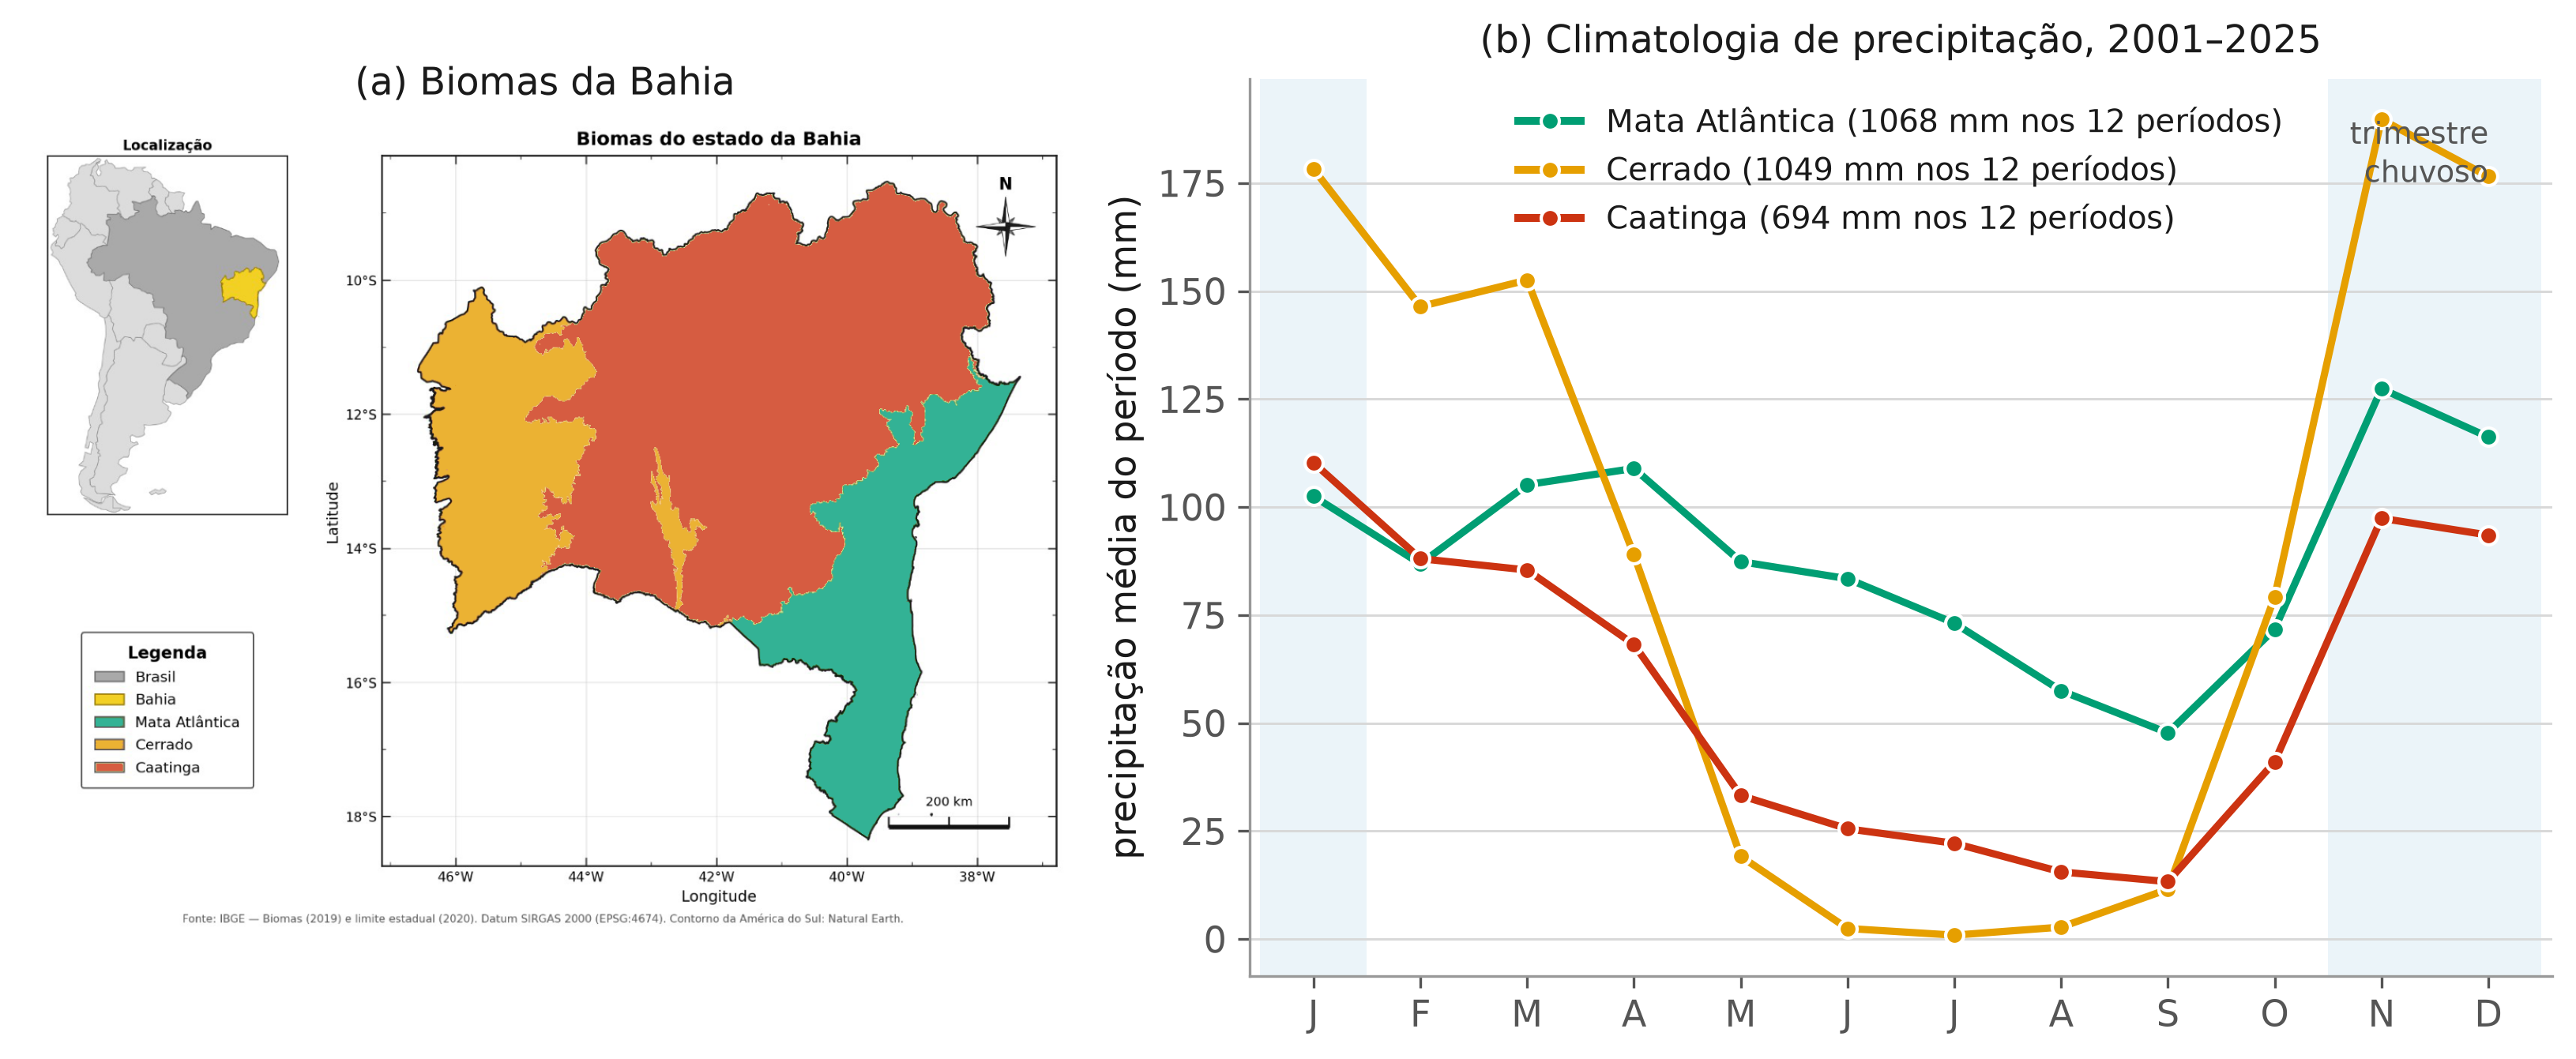
\includegraphics[width=\linewidth]{figs/fig1_area_estudo.png}
\caption{(a) Distribuição dos biomas Mata Atlântica, Cerrado e Caatinga no Estado da Bahia \citep[limites de][]{ibge2019}. (b) Precipitação média de cada mês civil por bioma na série de 2001 a 2025, com o trimestre climatologicamente mais chuvoso sombreado.}
\label{fig:area}
\end{figure}

\subsection{Dados}

A série mensal cobre janeiro de 2001 a setembro de 2025, com 297 períodos por bioma. Cada período é uma janela fixa de quatro compósitos consecutivos de oito dias, atribuída ao mês civil que contém a maior parte de seus dias: a janela de janeiro, por exemplo, reúne os compósitos iniciados em 27 de dezembro e em 1, 9 e 17 de janeiro. Cada janela abrange cerca de 32 dias, de modo que os períodos aqui chamados mensais não são meses civis estritos, e é ao mês de referência de cada janela que se associa a fase do ENSO. A fotossíntese líquida (PSN) provém do MOD17A2HGF C6.1 \citep{running2021gpp}; a evapotranspiração real (EV) e a potencial, do MOD16A2GF C6.1 \citep{running2021et}; a temperatura diurna da superfície (TST), do MOD11A2 C6.1 \citep{wan2021}; e a precipitação (PRE), do GPM IMERG Final Run V07 \citep{huffman2023}. O índice de disponibilidade hídrica (WAI) é a razão entre evapotranspiração real e potencial. As médias espaciais foram calculadas sobre os pixels válidos de cada bioma no Google Earth Engine \citep{gorelick2017}. A produtividade primária líquida anual do MOD17A3HGF é usada apenas como verificação de consistência na escala anual; todos os resultados mensais referem-se à PSN.

O Índice Oceânico Niño (ONI) foi obtido da tabela completa do Climate Prediction Center da NOAA \citep{noaacpc2025}. A classificação das fases segue o critério oficial: El Niño quando o ONI permanece em $+0{,}5$~$^{\circ}$C ou acima por cinco trimestres consecutivos sobrepostos, La Niña quando permanece em $-0{,}5$~$^{\circ}$C ou abaixo pelo mesmo intervalo, e Neutro nos demais casos. A série completa do índice desde 1950 foi usada na classificação, de modo que episódios iniciados antes de 2001 fossem reconhecidos.

\subsection{Anomalias}

Para cada variável e bioma, a climatologia é a média do mês civil correspondente ao longo de toda a série, e a anomalia é expressa em porcentagem dessa média. A remoção do ciclo anual é necessária porque as fases do ENSO não se distribuem uniformemente pelo calendário: os meses de El Niño representam de 10,5\% a 11,8\% da amostra entre novembro e fevereiro, mas apenas de 3,9\% a 5,3\% entre maio e julho, ao passo que os meses neutros seguem a distribuição inversa (4,0\% e 12,8\%, respectivamente). Uma comparação sobre valores brutos confundiria, portanto, fase e estação.

\subsection{Comparação entre fases}

A anomalia de cada fase ativa foi comparada à dos meses neutros pelo teste de Mann-Whitney, e as três fases pelo teste de Kruskal-Wallis, com o tamanho de efeito $\varepsilon^2$. A homogeneidade da dispersão foi avaliada pelo teste de Fligner-Killeen e a frequência de extremos por um teste qui-quadrado sobre a proporção de meses abaixo do percentil 10 e acima do percentil 90 da própria série de anomalias. Os valores de $p$ de cada família de testes foram corrigidos pelo procedimento de Benjamini-Hochberg, controlando a taxa de falsas descobertas em 5\% \citep{benjamini1995}.

\subsection{Estratificação sazonal}

O canal hídrico só pode operar quando há chuva a ser modulada, e o ENSO tem seu pico no verão austral. Por essa razão física, definida antes de examinar o desfecho, a comparação entre fases foi repetida em dois recortes sazonais, definidos pela climatologia de precipitação de cada bioma: o trimestre civil consecutivo de maior precipitação média e o de menor. O trimestre seco funciona como controle negativo, no sentido de que uma associação transmitida pelo canal hídrico da estação chuvosa deve estar ausente nele. Nesse recorte, a unidade amostral é o episódio, conforme a Seção~2.9, e a correção de Benjamini-Hochberg foi aplicada à família dos seis testes de cada trimestre, com a família dos doze testes reportada como análise de sensibilidade. Detectar associação em um trimestre e não no outro não estabelece, porém, que os dois difiram. Calculou-se por isso o contraste direto entre eles, como diferença das diferenças, isto é, a diferença entre a fase e os meses neutros no trimestre chuvoso menos essa mesma diferença no trimestre seco, com o mesmo bootstrap em blocos e reamostrando os mesmos episódios simultaneamente nos dois trimestres, de modo que o contraste seja pareado por episódio.

\subsection{Escalas de resposta temporal}

Duas escalas temporais foram examinadas. A primeira é a resposta ao forçante remoto, avaliada pela correlação de Spearman entre o ONI do mês $t$ e a anomalia de PSN do mês $t+L$, para $L$ de 0 a 12 meses. A segunda é a janela sobre a qual cada bioma integra a água recebida: para cada janela de 1 a 12 períodos calculou-se a chuva acumulada nos períodos terminados em $t$, sua anomalia em relação à climatologia da mesma janela, e a correlação de Spearman com a anomalia de PSN em $t$. A janela de maior associação é uma medida empírica de quanto tempo o sistema integra a água disponível. Em ambas as escalas os meses são tratados como independentes; os coeficientes descrevem a forma das curvas e não sustentam teste individual, e não foram submetidos a correção para comparações múltiplas.

\subsection{Experimento de perturbação com o modelo}

Para verificar se as anomalias climáticas observadas em cada fase são compatíveis, em direção e magnitude, com as anomalias observadas de PSN, usou-se o modelo de regressão polinomial de grau 2 com regularização de Ridge ajustado para os mesmos biomas e período \citep{oliveira2026, hoerl1970}. O modelo prevê a PSN com os preditores em sua climatologia mensal e, alternativamente, com cada preditor (ou todos) deslocado pela anomalia média observada em cada fase; a diferença entre as duas predições, em porcentagem da PSN climatológica, é a resposta que o modelo atribui a cada canal. O modelo foi ajustado aos mesmos dados sobre os quais o experimento é conduzido, de modo que o procedimento mede a compatibilidade entre as anomalias observadas e a resposta que o modelo lhes atribui, e não a fração da resposta causalmente transmitida por cada variável. Nenhuma inferência causal é pretendida.

\subsection{Variabilidade interanual}

A PSN anual é a soma dos períodos de cada ano. A tendência foi estimada pelo declive de Sen \citep{sen1968} e testada por Mann-Kendall \citep{mann1945}. A soma anual foi comparada, por correlação de Pearson, à produtividade primária líquida anual do MOD17A3HGF para as mesmas máscaras de bioma, como verificação de consistência entre dois produtos da mesma família. O ano de 2025, com nove períodos disponíveis, foi excluído do cálculo de tendência.

\subsection{O episódio como unidade amostral}

Os testes da Seção~2.4 supõem que as observações de cada grupo sejam independentes. Os meses de uma mesma fase não o são: pertencem a um número reduzido de episódios, cada um com vários meses consecutivos, e tanto o forçante oceânico quanto a resposta da vegetação são autocorrelacionados dentro de um episódio. A unidade efetiva de amostragem é o episódio.

A estatística de interesse, a diferença entre a anomalia percentual média de uma fase ativa e a dos meses neutros, foi por isso acompanhada de dois intervalos de confiança de 95\%, ambos por percentis de 10.000 reamostragens com a mesma semente: um por bootstrap i.i.d., sorteando meses com reposição dentro de cada grupo, que é o esquema implícito nos testes convencionais; e outro por bootstrap em blocos, sorteando com reposição sequências contíguas inteiras de meses da mesma fase \citep{kunsch1989, politis1994}. Os blocos foram definidos como corridas contíguas de meses na mesma fase oficial, sem imposição de comprimento: cada bloco é um episódio do ENSO tal como a NOAA o delimita. Os dois esquemas foram aplicados à PSN e aos quatro preditores nos três biomas, totalizando 30 testes em cada um, e seus valores de $p$ foram submetidos ao mesmo procedimento de Benjamini-Hochberg da Seção~2.4.

Todas as análises foram feitas em Python 3.11 com \texttt{numpy}, \texttt{pandas}, \texttt{scipy} e \texttt{scikit-learn}.

\section{Resultados}

\subsection{Composição das fases}

Dos 297 períodos da série, 76 foram classificados como El Niño, 72 como La Niña e 149 como neutros. Esses meses distribuem-se em poucas sequências contíguas: 8 episódios de El Niño, 9 sequências de La Niña (uma delas truncada no início da série, em janeiro e fevereiro de 2001) e 17 intervalos neutros (Tabela~\ref{tab:fases}), com duração entre 2 e 20 meses e mediana de 8 meses.

\begin{table}[width=\linewidth,cols=5,pos=!ht]
\caption{Composição das fases do ENSO na série mensal de 2001 a 2025, segundo o critério oficial da NOAA.}
\label{tab:fases}
\begin{tabular*}{\tblwidth}{@{}lrrrr@{}}
\toprule
Fase & Meses & Sequências & \multicolumn{2}{c}{Duração (meses)} \\
\cmidrule(l){4-5}
 & & & mediana & mín--máx \\
\midrule
El Niño & 76  & 8  & 8,5 & 5--20 \\
Neutro  & 149 & 17 & 7   & 1--30 \\
La Niña & 72  & 9  & 7   & 2--17 \\
\midrule
Total   & 297 & 34 & --- & --- \\
\bottomrule
\end{tabular*}
\end{table}

A Figura~\ref{fig:episodios} mostra a série de anomalias de PSN dos três biomas com os episódios sombreados. A variabilidade mensal é alta em todos os biomas, com amplitude de cerca de $\pm 40\%$ na Mata Atlântica e de $\pm 90\%$ no Cerrado, e o El Niño de 2014--2016 coincide com as anomalias negativas mais profundas da Mata Atlântica.

\begin{figure}[pos=!ht]
\centering
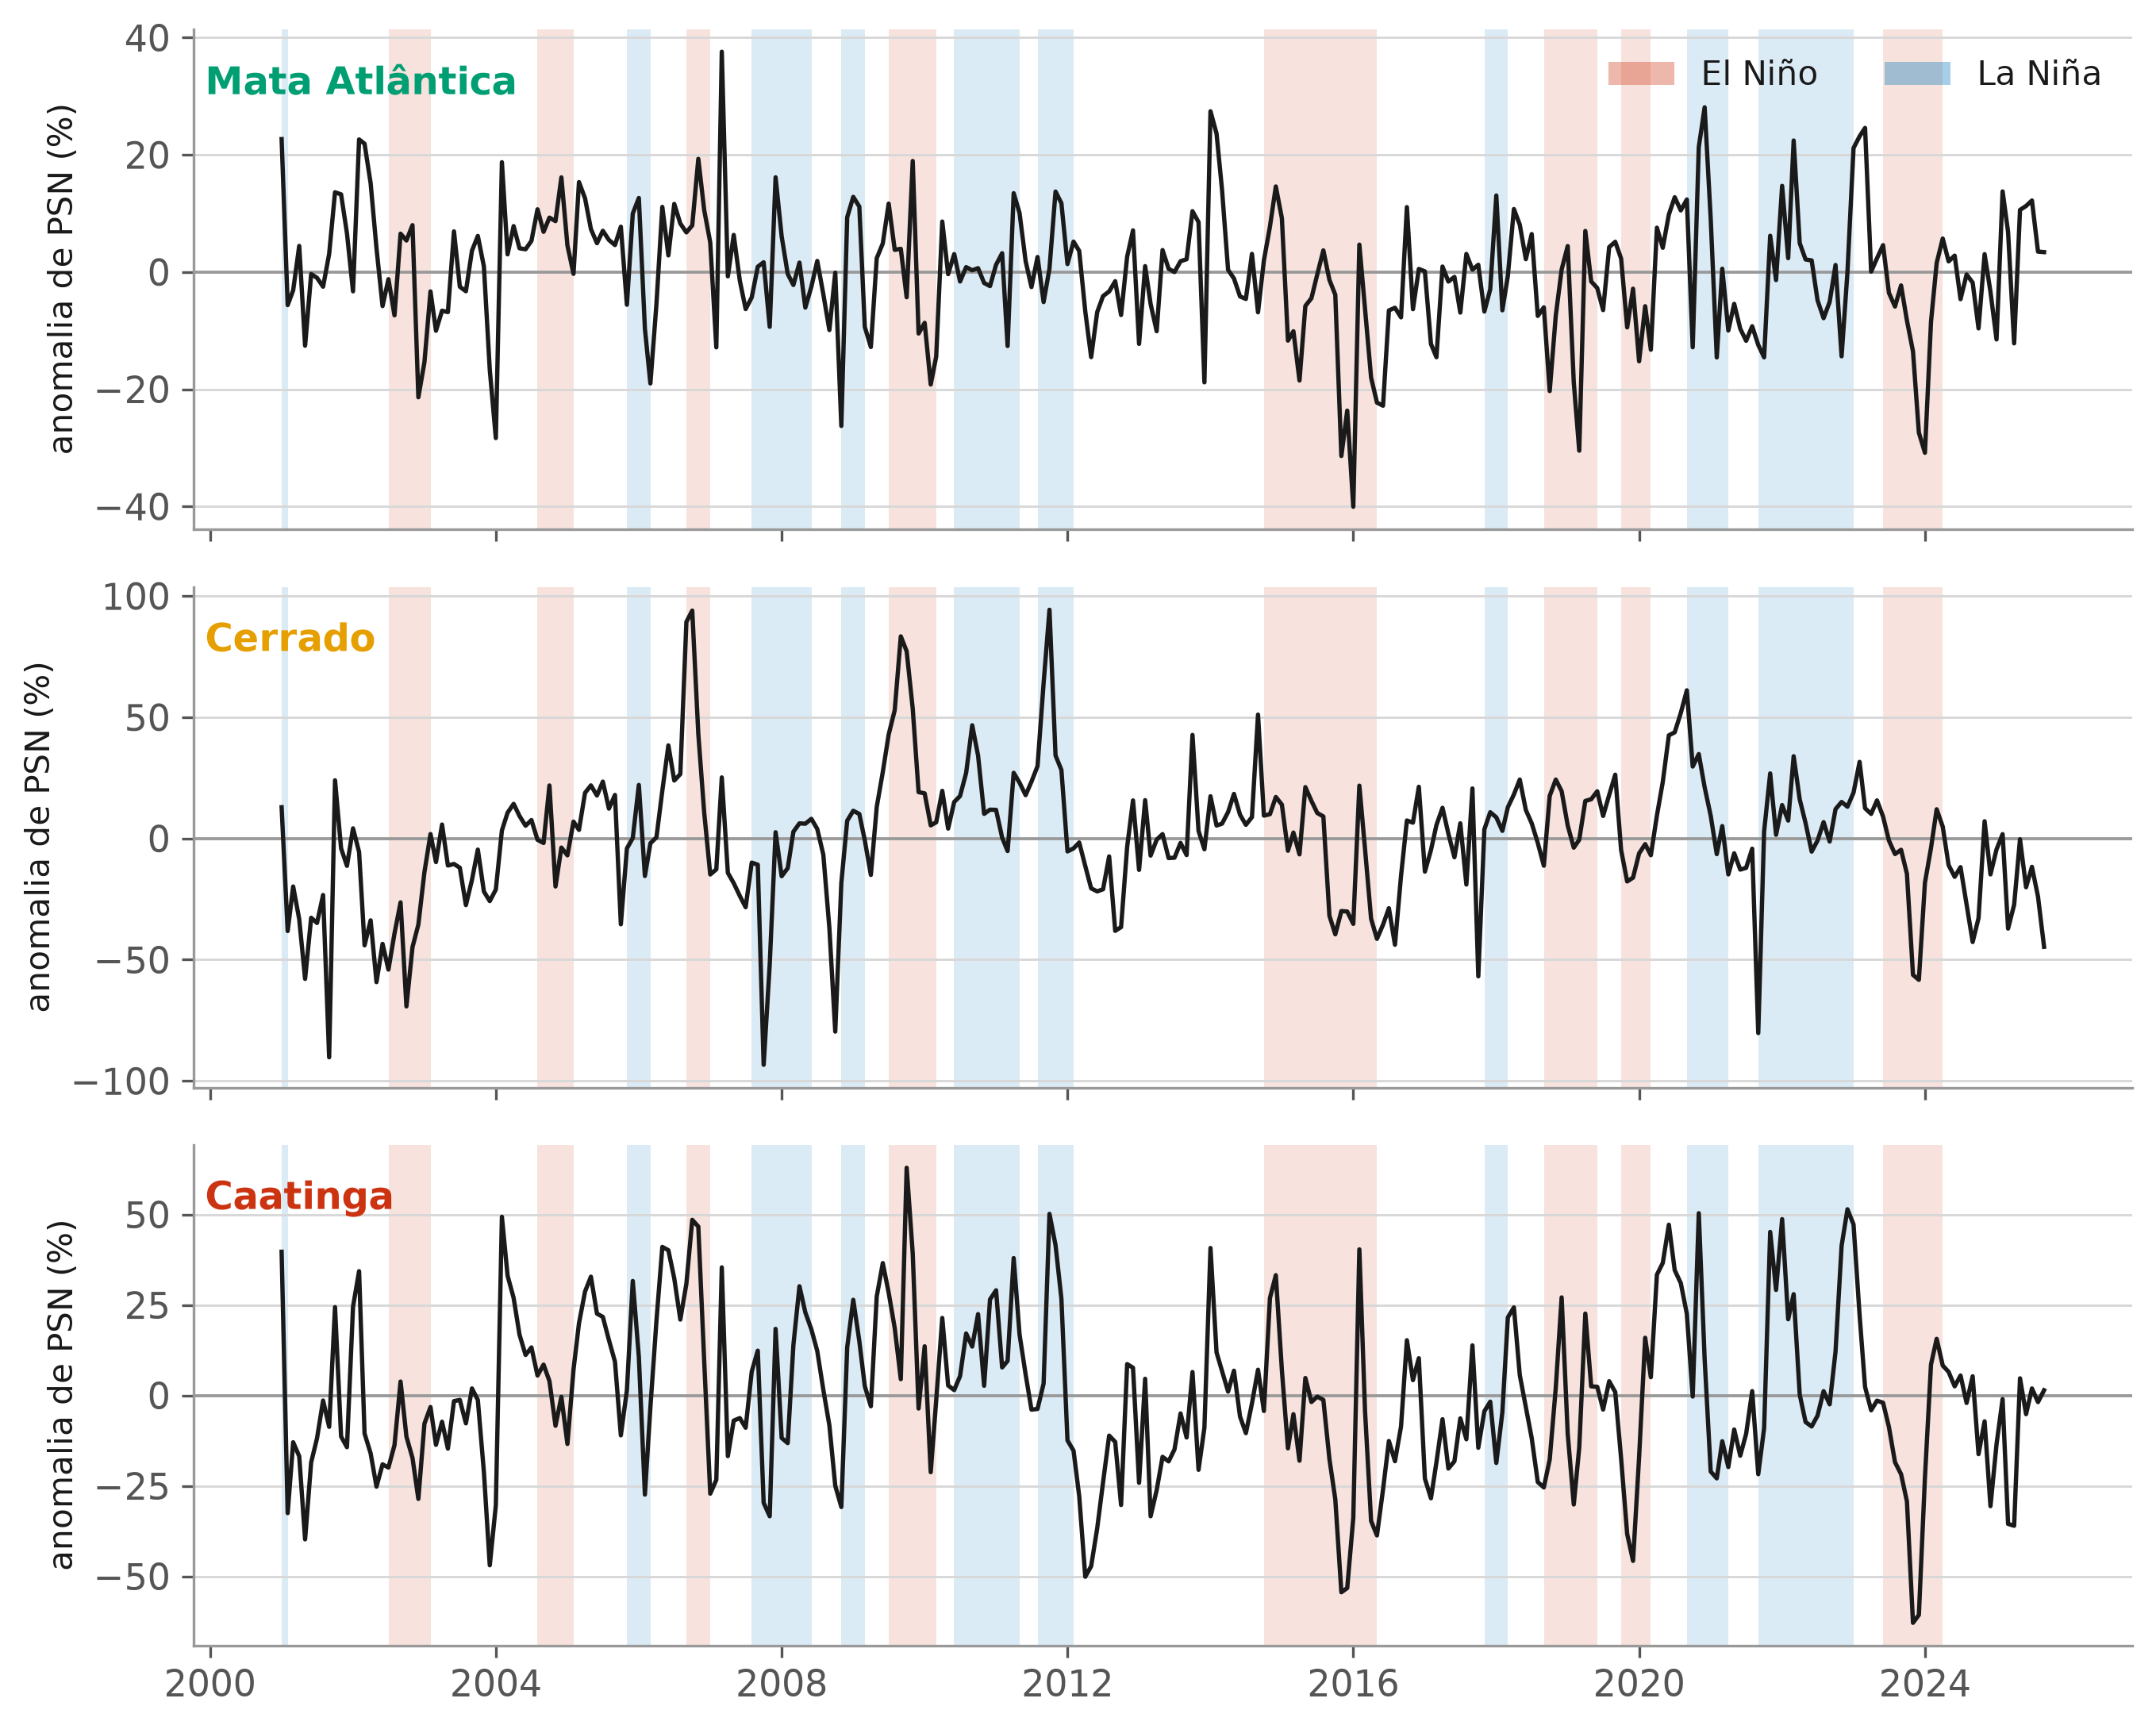
\includegraphics[width=\linewidth]{figs/fig1_episodios.png}
\caption{Anomalia percentual mensal da fotossíntese líquida nos três biomas entre 2001 e 2025, com os episódios de El Niño e de La Niña sombreados. As escalas verticais diferem entre os painéis.}
\label{fig:episodios}
\end{figure}

\subsection{Mata Atlântica: o sinal chega como anomalia térmica}

\begin{table*}[width=\textwidth,cols=7,pos=t]
\caption{Anomalia percentual média de cada fase ativa em relação aos meses neutros, com o valor de $p$ do teste de Mann-Whitney. Em negrito, os resultados que sobreviveram à correção de Benjamini-Hochberg (taxa de falsas descobertas de 5\%).}
\label{tab:convencional}
\begin{tabular*}{\tblwidth}{@{}llrrrr@{}}
\toprule
Bioma & Variável & \multicolumn{2}{c}{El Niño} & \multicolumn{2}{c}{La Niña} \\
\cmidrule(lr){3-4}\cmidrule(l){5-6}
 & & $\Delta$ (p.p.) & $p$ & $\Delta$ (p.p.) & $p$ \\
\midrule
Mata Atlântica & PSN & $\mathbf{-5{,}44}$ & \textbf{0,010} & $-0{,}08$ & 0,794 \\
               & EV  & $-1{,}52$ & 0,488 & $+1{,}37$ & 0,359 \\
               & PRE & $-5{,}28$ & 0,181 & $-1{,}27$ & 0,888 \\
               & TST & $\mathbf{+3{,}07}$ & \textbf{$<$0,001} & $-0{,}50$ & 0,322 \\
               & WAI & $-2{,}49$ & 0,189 & $+2{,}44$ & 0,182 \\
\addlinespace
Cerrado        & PSN & $+5{,}26$ & 0,375 & $\mathbf{+11{,}75}$ & \textbf{0,001} \\
               & EV  & $+7{,}51$ & 0,080 & $\mathbf{+10{,}22}$ & \textbf{$<$0,001} \\
               & PRE & $+7{,}91$ & 0,875 & $-7{,}73$ & 0,461 \\
               & TST & $+1{,}35$ & 0,217 & $-1{,}11$ & 0,050 \\
               & WAI & $+7{,}70$ & 0,245 & $\mathbf{+13{,}99}$ & \textbf{$<$0,001} \\
\addlinespace
Caatinga       & PSN & $-3{,}28$ & 0,458 & $\mathbf{+10{,}45}$ & \textbf{0,002} \\
               & EV  & $+0{,}34$ & 0,630 & $\mathbf{+10{,}85}$ & \textbf{0,003} \\
               & PRE & $+2{,}54$ & 0,761 & $+4{,}69$ & 0,837 \\
               & TST & $+1{,}51$ & 0,105 & $\mathbf{-2{,}14}$ & \textbf{0,013} \\
               & WAI & $+0{,}43$ & 0,534 & $\mathbf{+12{,}47}$ & \textbf{0,002} \\
\bottomrule
\end{tabular*}
\end{table*}

Na Mata Atlântica, a variável climática mais sensível às fases do ENSO foi a temperatura da superfície: nos meses de El Niño ela ficou 3,1~p.p.\ acima do normal da época, cerca de 0,9~$^{\circ}$C ($p < 0{,}001$), com 25\% desses meses no decil mais quente da série contra 5\% dos meses neutros (Tabela~\ref{tab:convencional}). A evapotranspiração e a precipitação não diferiram na posição central.

A PSN acompanhou esse aquecimento de uma forma particular, que o valor médio esconde. As medianas brutas são praticamente iguais nas três fases (133,3, 134,3 e 133,8~gC~m$^{-2}$ por período), mas, removido o ciclo anual, os meses de El Niño apresentaram anomalia média de $-5{,}4$~p.p.\ ($p = 0{,}010$) e 22,4\% deles ficaram abaixo do percentil 10 da série, contra 4,7\% dos meses neutros e 8,3\% dos de La Niña ($p = 0{,}0004$). O mínimo observado sob El Niño (79,0~gC~m$^{-2}$) fica 15 unidades abaixo do mínimo dos meses neutros (94,4). Nesse bioma, portanto, a associação do El Niño com a produtividade concentra-se na cauda inferior da distribuição, e não no seu centro. A La Niña não produziu resposta na Mata Atlântica em nenhuma das propriedades avaliadas ($-0{,}1$~p.p.; $p = 0{,}794$). A correlação com o ONI foi máxima com dois meses de defasagem ($\rho = -0{,}16$).

\subsection{Cerrado: sinal hídrico e associação persistente}

No Cerrado o sinal apareceu nas variáveis que integram a água efetivamente utilizada pela vegetação, e na fase fria. Nos meses de La Niña a evapotranspiração ficou 10,2~p.p.\ acima do normal da época e o índice de disponibilidade hídrica 14,0~p.p.\ acima (ambos $p < 0{,}001$), enquanto nos meses de El Niño as anomalias correspondentes não foram significativas. A PSN acompanhou, com anomalia média de $+11{,}7$~p.p.\ em La Niña ($p = 0{,}001$) e de $+5{,}3$~p.p.\ em El Niño ($p = 0{,}375$). A associação com a fase fria desloca a distribuição inteira: o primeiro quartil sobe de 65,1 para 85,8~gC~m$^{-2}$ por período.

A precipitação do próprio período não apresentou diferença detectável entre fases. As médias brutas sugeririam o contrário: são 123~mm por período em La Niña e 107~mm em El Niño, contra 59~mm nos meses neutros. Como as duas fases ativas superam a neutra na mesma direção, porém, o que se observa é o efeito de calendário antecipado na Seção~2.3, e a diferença de 64~mm entre La Niña e meses neutros cai para 8~mm quando o ciclo anual é removido. O sinal do ENSO associado à produtividade desse bioma aparece, assim, nas variáveis que integram a água disponível ao longo de semanas, e não no total precipitado no período.

A associação com o ONI foi fraca e notavelmente persistente, como detalhado na Seção~3.5.

\subsection{Caatinga: sinal hídrico e resposta em fase}

Na Caatinga o quadro repetiu-se quanto às variáveis, mas não quanto ao tempo. Nos meses de La Niña a evapotranspiração ficou 10,9~p.p.\ acima do normal ($p = 0{,}003$), o índice de disponibilidade hídrica 12,5~p.p.\ acima ($p = 0{,}002$), a temperatura 2,1~p.p.\ abaixo ($p = 0{,}013$) e a PSN 10,4~p.p.\ acima ($p = 0{,}002$; mediana de 94,6 contra 82,4~gC~m$^{-2}$ nos meses neutros). Como no Cerrado, a precipitação do próprio período não diferiu entre fases. Nos meses de El Niño a PSN ficou 3,3~p.p.\ abaixo do normal, diferença não significativa ($p = 0{,}458$), ainda que 14,5\% desses meses tenham caído no decil mais baixo, contra 10,1\% dos neutros e 5,6\% dos de La Niña.

A diferença em relação ao Cerrado está na estrutura temporal, tratada na seção seguinte.

\subsection{Escalas de resposta temporal}

As duas escalas examinadas separam os biomas de maneiras distintas (Figura~\ref{fig:temporal}). A associação com o forçante remoto é fraca em todos eles: a correlação com o ONI não ultrapassa $\rho = -0{,}19$, ou 3,6\% da variância das anomalias. Dentro dessa faixa estreita, a Caatinga apresenta o máximo em fase ($L = 0$) e decai a partir de cinco meses; a Mata Atlântica tem máximo em $L = 2$; e o Cerrado mantém valores praticamente constantes entre $L = 1$ e $L = 12$, sem pico definido.

A associação com a água acumulada é de outra ordem de grandeza, entre $\rho = 0{,}48$ e $0{,}67$, e separa os biomas com nitidez. Na janela de um período, a Caatinga já apresenta $\rho = 0{,}32$, contra 0,09 no Cerrado e $-0{,}02$ na Mata Atlântica: é o único bioma cuja produtividade se associa à chuva do próprio período. Seu máximo ocorre em quatro períodos ($\rho = 0{,}67$) e cai para 0,46 em doze, retendo 69\% do pico. O Cerrado tem máximo em cinco períodos ($\rho = 0{,}55$) e ainda retém 0,49 em doze, ou 88\% do pico, a curva mais achatada dos três. A Mata Atlântica tem máximo em cinco períodos ($\rho = 0{,}48$) e retém 72\%.

O contraste entre os dois painéis da Figura~\ref{fig:temporal} é, em si, informativo: a produtividade desses biomas associa-se muito mais à água efetivamente acumulada do que ao índice oceânico que a modula.

\begin{figure}[pos=!ht]
\centering
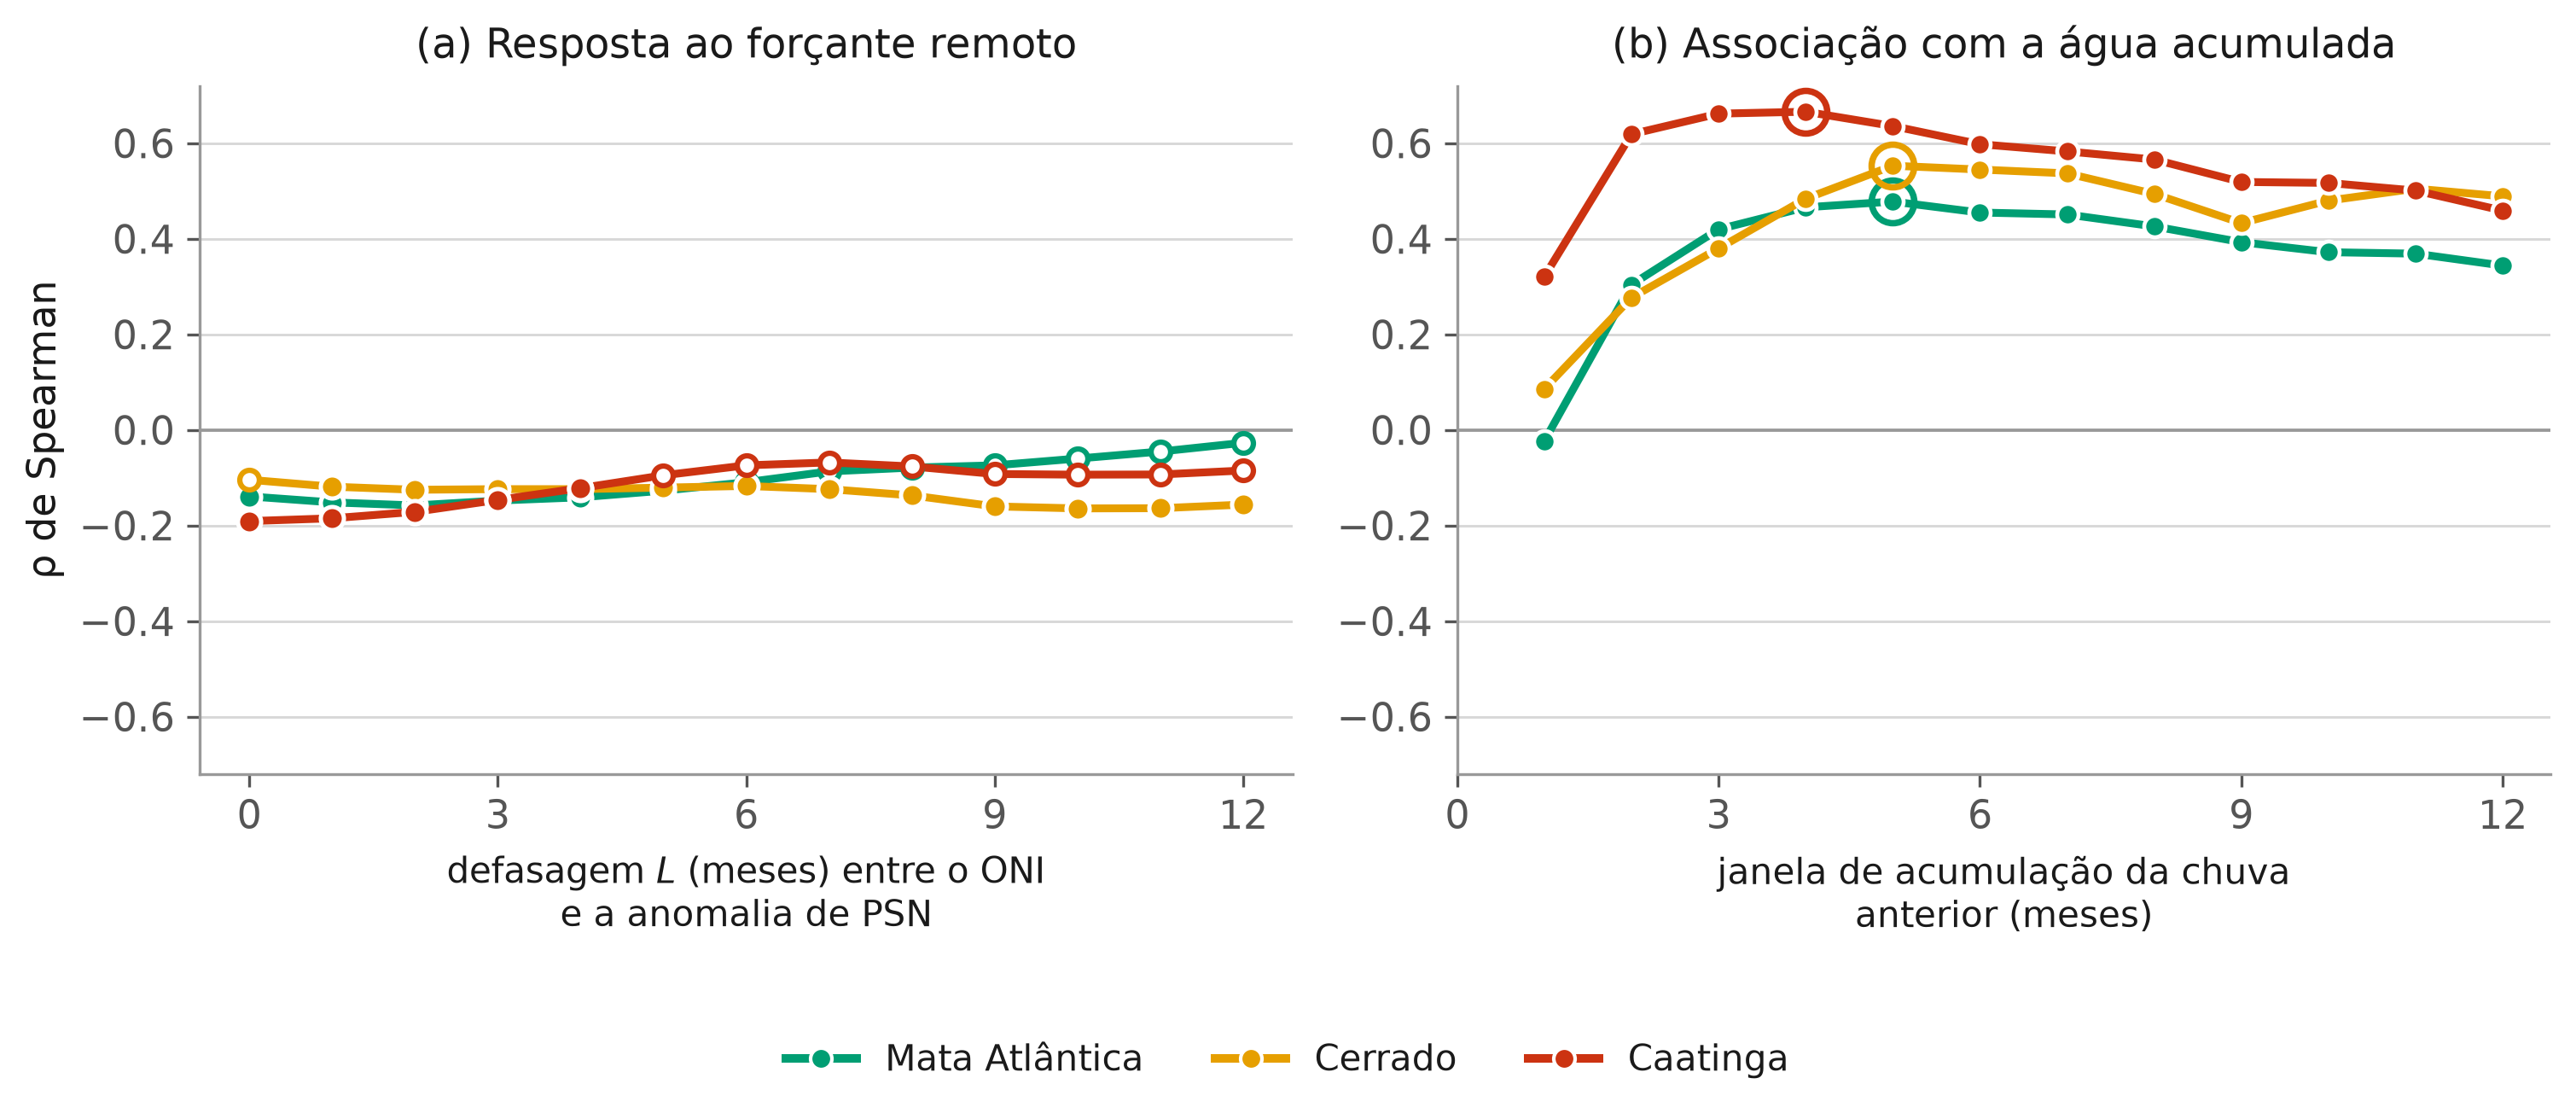
\includegraphics[width=\linewidth]{figs/fig3_resposta_temporal.png}
\caption{(a) Correlação de Spearman entre o ONI do mês $t$ e a anomalia de PSN do mês $t+L$; os símbolos preenchidos indicam $p < 0{,}05$ sob a premissa de meses independentes. (b) Correlação entre a anomalia de PSN e a anomalia da chuva acumulada nos períodos anteriores, por janela de acumulação; o círculo maior assinala a janela de maior associação em cada bioma. As duas escalas verticais são iguais.}
\label{fig:temporal}
\end{figure}

\subsection{Confinamento sazonal da resposta}

A associação com a La Niña concentra-se na estação chuvosa e desaparece na seca (Tabela~\ref{tab:sazonal}, Figura~\ref{fig:sazonal}). O trimestre climatologicamente mais chuvoso é novembro--dezembro--janeiro nos três biomas. Nesse recorte, e com o episódio como unidade amostral, a anomalia de PSN associada à La Niña foi de $+25{,}0$~p.p.\ na Caatinga (IC95\% $+8{,}3$ a $+43{,}3$; $q = 0{,}005$), $+11{,}9$~p.p.\ no Cerrado (IC95\% $+0{,}7$ a $+23{,}9$; $q = 0{,}073$) e $+7{,}4$~p.p.\ na Mata Atlântica (IC95\% $+1{,}4$ a $+15{,}6$; $q = 0{,}034$). A magnitude cresce, portanto, na direção do polo semiárido do gradiente.

No trimestre mais seco de cada bioma nenhuma associação foi detectada, em nenhuma fase, com todos os valores de $q$ acima de 0,25. O El Niño não produziu associação detectável em nenhum dos dois recortes.

Detectar associação em um trimestre e não no outro não estabelece, contudo, que os dois difiram. O contraste direto entre os trimestres, pareado por episódio, é conclusivo em apenas um dos biomas: na Mata Atlântica ele é de $+10{,}9$~p.p.\ (IC95\% $+3{,}2$ a $+20{,}4$; $p = 0{,}004$), ou seja, a resposta à La Niña é de fato maior na estação chuvosa do que na seca. Na Caatinga o contraste é o maior em magnitude, $+20{,}5$~p.p., mas não se distingue de zero (IC95\% $-5{,}0$ a $+47{,}3$; $p = 0{,}142$), porque a estimativa do trimestre seco é ela própria imprecisa. No Cerrado o contraste é praticamente nulo ($-0{,}6$~p.p.; $p = 0{,}923$). O confinamento sazonal da resposta é, portanto, um padrão observado nos três biomas e uma diferença estabelecida apenas na Mata Atlântica.

Duas ressalvas acompanham esses resultados. A primeira é que a correção de Benjamini-Hochberg foi aplicada à família dos seis testes de cada trimestre; estendida aos doze testes dos dois trimestres, apenas a Caatinga permanece ($q = 0{,}011$), enquanto a Mata Atlântica passa a $q = 0{,}068$. A segunda é que o trimestre chuvoso coincide com o pico sazonal do ENSO, o que faz parte do próprio canal examinado; como as anomalias são calculadas em relação à climatologia do mesmo mês civil, essa coincidência não introduz o efeito de calendário discutido na Seção~2.3.

\begin{table}[width=\linewidth,cols=6,pos=!ht]
\caption{Anomalia de PSN associada a cada fase, em relação aos meses neutros, no trimestre climatologicamente mais chuvoso e mais seco de cada bioma, e contraste direto entre os dois trimestres. Unidade amostral: o episódio. $q$ refere-se à família dos seis testes de cada trimestre.}
\label{tab:sazonal}
\begin{tabular*}{\tblwidth}{@{}llrrrrr@{}}
\toprule
Bioma & Fase & \multicolumn{2}{c}{Chuvoso} & \multicolumn{2}{c}{Seco} & Contraste \\
\cmidrule(lr){3-4}\cmidrule(lr){5-6}
 & & $\Delta$ & $q$ & $\Delta$ & $q$ & $\Delta$ ($p$) \\
\midrule
Mata Atlântica & El Niño & $-3{,}13$  & 0,806 & $-0{,}40$  & 0,866 & $-2{,}7$ (0,586) \\
               & La Niña & $\mathbf{+7{,}42}$  & \textbf{0,034} & $-3{,}43$  & 0,356 & $\mathbf{+10{,}9}$ \textbf{(0,004)} \\
\addlinespace
Cerrado        & El Niño & $-2{,}90$  & 0,806 & $+7{,}56$  & 0,832 & $-10{,}5$ (0,380) \\
               & La Niña & $+11{,}88$ & 0,073 & $+12{,}49$ & 0,356 & $-0{,}6$ (0,923) \\
\addlinespace
Caatinga       & El Niño & $-2{,}47$  & 0,806 & $-1{,}24$  & 0,866 & $-1{,}2$ (0,885) \\
               & La Niña & $\mathbf{+25{,}00}$ & \textbf{0,005} & $+4{,}47$  & 0,814 & $+20{,}5$ (0,142) \\
\bottomrule
\end{tabular*}
\end{table}

\begin{figure}[pos=!ht]
\centering
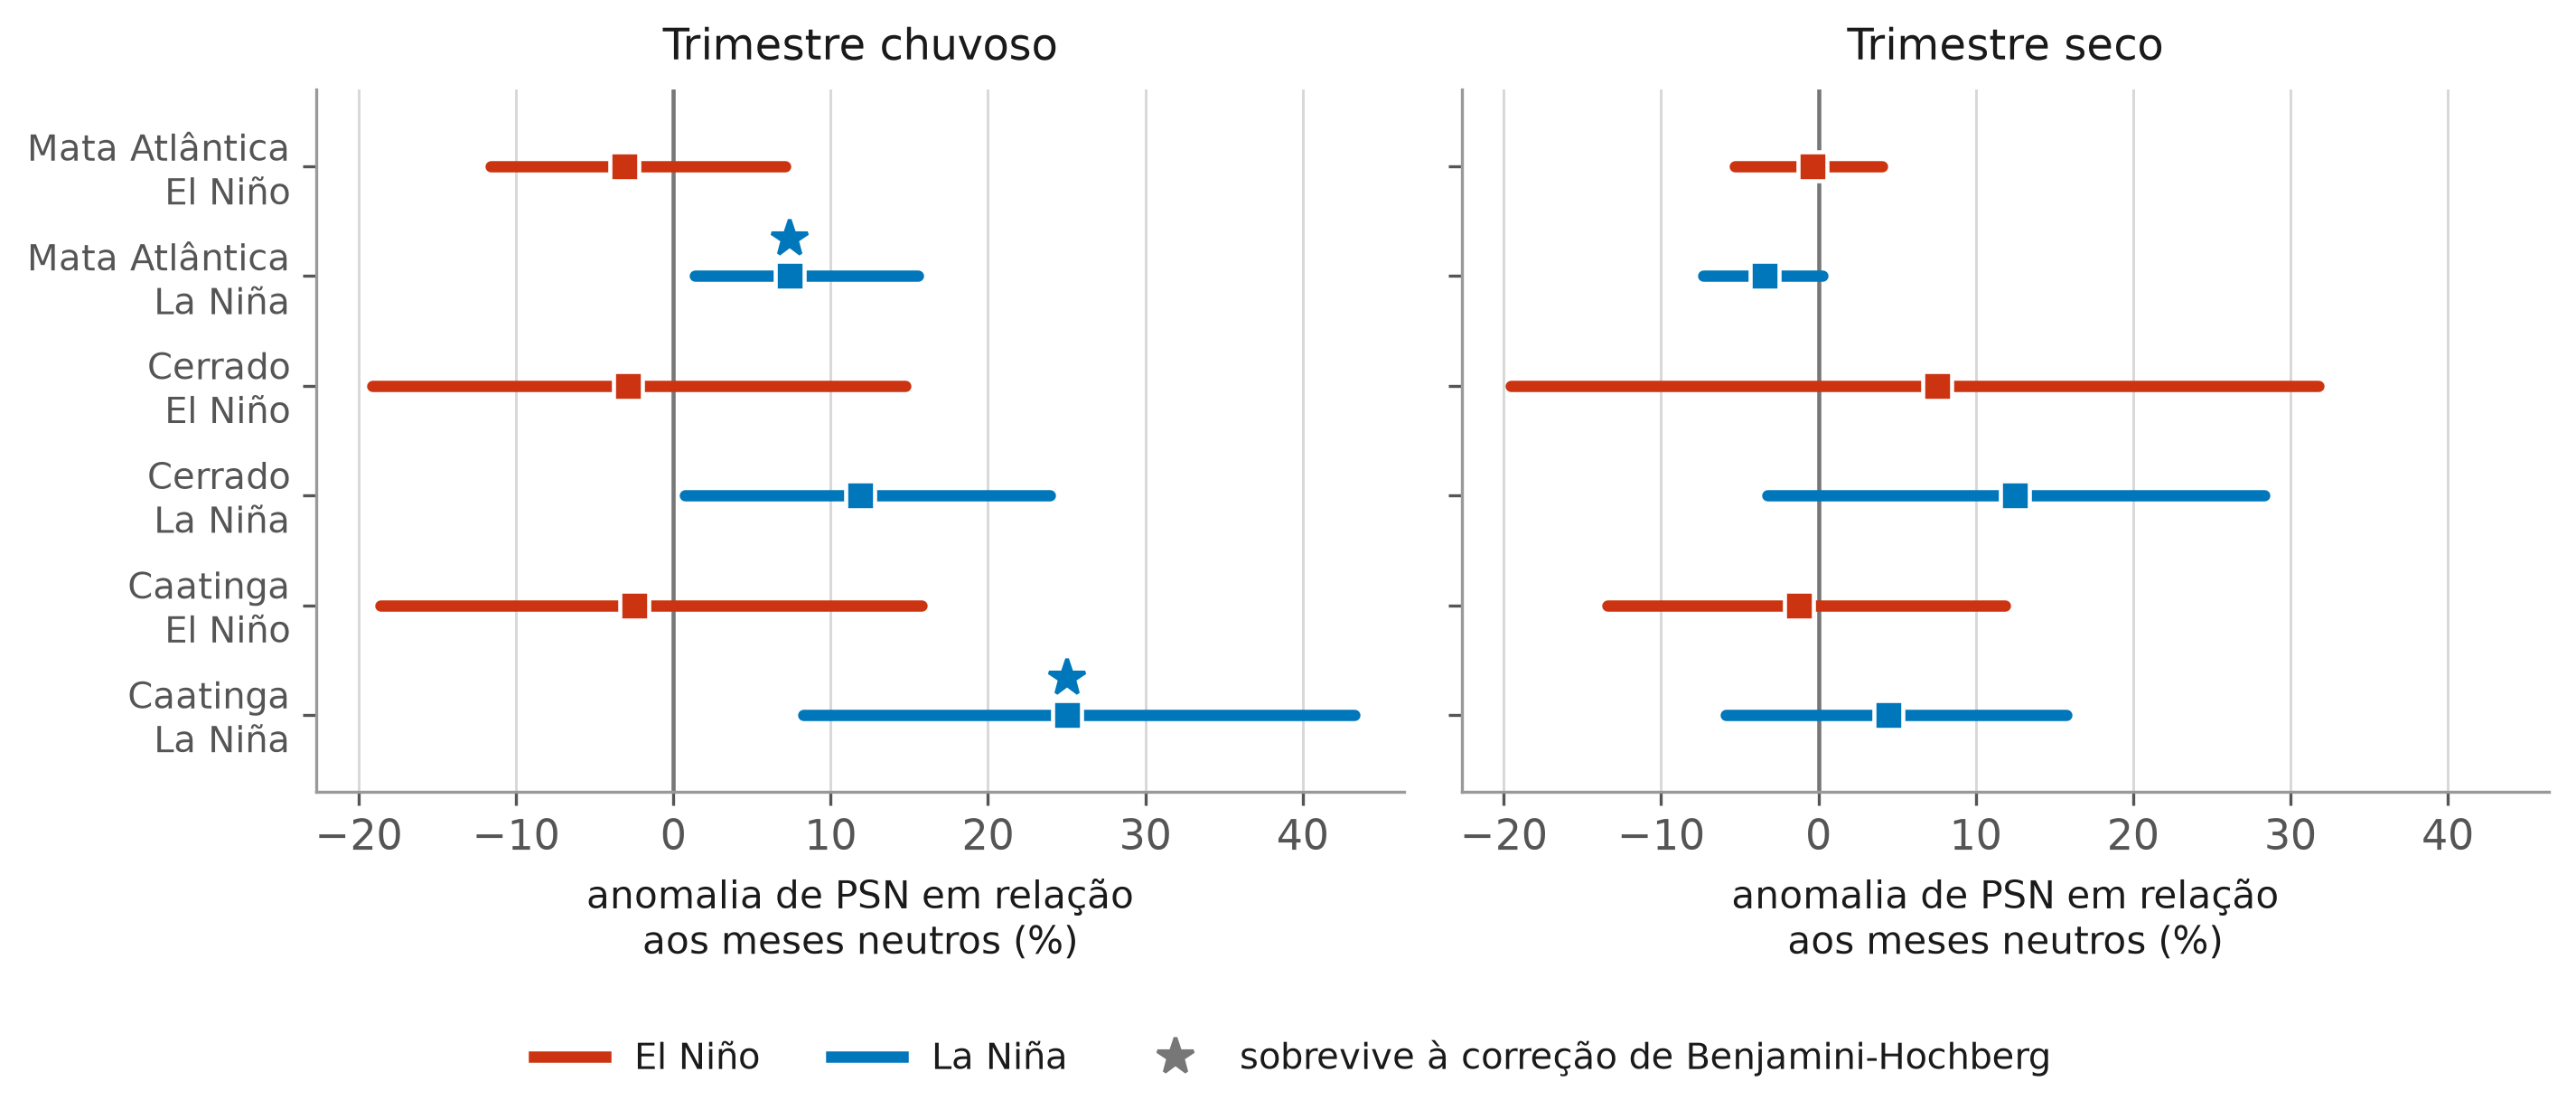
\includegraphics[width=\linewidth]{figs/fig4_sazonal.png}
\caption{Anomalia de PSN de cada fase em relação aos meses neutros, no trimestre mais chuvoso e no mais seco de cada bioma, com intervalos de confiança de 95\% por bootstrap em blocos sobre episódios.}
\label{fig:sazonal}
\end{figure}

\subsection{Compatibilidade entre as anomalias climáticas e a resposta da PSN}

Impondo ao modelo as anomalias médias observadas em cada fase, a resposta predita reproduz boa parte da observada nas combinações de maior magnitude (Tabela~\ref{tab:perturbacao}). Na Caatinga em La Niña, o modelo prediz $+9{,}8\%$ contra $+10{,}4\%$ observados; no Cerrado na mesma fase, $+8{,}0\%$ contra $+11{,}7\%$; e na Mata Atlântica em El Niño, $-3{,}1\%$ contra $-5{,}4\%$.

A decomposição por canal mostra que a via difere entre os biomas, mas também que os canais não são separáveis nem aditivos. Na Mata Atlântica em El Niño, deslocar apenas a temperatura produz $-2{,}8\%$, o maior canal isolado, contra $-2{,}4\%$ da evapotranspiração e $+2{,}0\%$ da disponibilidade hídrica, que atua em sentido oposto; o canal térmico corresponde, assim, a cerca de 90\% da resposta que o modelo atribui ao conjunto e a cerca de metade da anomalia observada, mas está a apenas 14\% do canal da evapotranspiração. Nos dois biomas sazonais a evapotranspiração domina: sozinha, produz $+11{,}6\%$ no Cerrado e $+9{,}0\%$ na Caatinga. No Cerrado, o canal isolado da evapotranspiração excede a resposta do conjunto, porque a precipitação e a disponibilidade hídrica atuam em sentido contrário dentro do modelo, reflexo da colinearidade entre evapotranspiração e disponibilidade hídrica já reportada nesse bioma \citep{oliveira2026}. Essas proporções descrevem a estrutura da resposta reproduzida pelo modelo e não medem transmissão causal.

\begin{table}[width=\linewidth,cols=6,pos=!ht]
\caption{Resposta da PSN predita pelo modelo quando lhe são impostas as anomalias médias observadas em cada fase, por canal e para o conjunto dos preditores, comparada à anomalia observada. Valores em porcentagem da PSN climatológica.}
\label{tab:perturbacao}
\begin{tabular*}{\tblwidth}{@{}llrrrr@{}}
\toprule
Bioma & Fase & Maior canal & Demais canais & Conjunto & Observado \\
\midrule
Mata Atlântica & El Niño & TST $-2{,}78$ & EV $-2{,}44$; WAI $+2{,}01$ & $-3{,}11$ & $-5{,}44$ \\
Mata Atlântica & La Niña & EV $+2{,}05$  & TST $+0{,}51$; WAI $-1{,}82$ & $+0{,}74$ & $-0{,}08$ \\
Cerrado        & El Niño & EV $+5{,}03$  & PRE $-0{,}08$; WAI $-0{,}41$ & $+4{,}48$ & $+5{,}26$ \\
Cerrado        & La Niña & EV $+11{,}62$ & PRE $-1{,}07$; WAI $-1{,}92$ & $+8{,}02$ & $+11{,}75$ \\
Caatinga       & El Niño & TST $-0{,}66$ & EV $-0{,}42$; PRE $-0{,}09$ & $-1{,}17$ & $-3{,}28$ \\
Caatinga       & La Niña & EV $+8{,}98$  & TST $+0{,}96$; PRE $-0{,}34$ & $+9{,}84$ & $+10{,}45$ \\
\bottomrule
\end{tabular*}
\end{table}

\subsection{Variabilidade interanual}

Nenhum dos três biomas apresentou tendência significativa da PSN anual entre 2001 e 2024 (Tabela~\ref{tab:interanual}). O declive de Sen foi negativo na Mata Atlântica ($-6{,}2\%$ no período) e positivo no Cerrado ($+11{,}3\%$) e na Caatinga ($+0{,}7\%$), mas os intervalos de confiança cruzam zero em todos os casos ($p = 0{,}070$, 0,333 e 0,941). Como verificação de consistência, a soma anual de PSN foi comparada à produtividade primária líquida anual do MOD17A3HGF para as mesmas máscaras, com correlação de Pearson entre 0,993 e 0,999.

A variabilidade interanual é muito desigual entre os biomas: o coeficiente de variação da PSN anual é de 4,6\% na Mata Atlântica, contra 15,0\% no Cerrado e 13,3\% na Caatinga. Os anos extremos não coincidem com as fases do ENSO de forma sistemática. O pior ano da Mata Atlântica, 2016, sucede o El Niño de 2014--2016, mas o melhor ano do Cerrado, 2009, é também um ano de El Niño, e o melhor da Caatinga, 2020, é um ano neutro. A escala anual mistura meses de fases distintas e é, por isso, menos nítida do que a análise mensal em anomalias.

\begin{table}[width=\linewidth,cols=6,pos=!ht]
\caption{Variabilidade interanual da PSN entre 2001 e 2024. O declive de Sen é expresso em porcentagem do período e testado por Mann-Kendall.}
\label{tab:interanual}
\begin{tabular*}{\tblwidth}{@{}lrrrrr@{}}
\toprule
Bioma & Média & CV & Sen & $p$ & Extremos \\
 & (gC~m$^{-2}$~ano$^{-1}$) & (\%) & (\%) & & (mín/máx) \\
\midrule
Mata Atlântica & 1.604 & 4,6  & $-6{,}2$  & 0,070 & 2016/2014 \\
Cerrado        & 1.157 & 15,0 & $+11{,}3$ & 0,333 & 2002/2009 \\
Caatinga       & 1.044 & 13,3 & $+0{,}7$  & 0,941 & 2012/2020 \\
\bottomrule
\end{tabular*}
\end{table}

\subsection{Robustez: o episódio como unidade amostral}

Repetindo a comparação agregada com o episódio como unidade, o sentido e a magnitude das anomalias não mudam, porque a estatística é a mesma, mas a precisão com que são estimadas diminui de forma apreciável. A largura mediana do intervalo de confiança passa de 12,9 para 23,1 pontos percentuais, um alargamento de 1,67 vez em mediana, que chega a 2,53 vezes. Dos 30 testes, 10 tinham intervalo excluindo o zero com o mês como unidade e 3 o mantêm com o episódio: o aquecimento da superfície da Mata Atlântica em El Niño ($p = 0{,}005$), a redução da PSN nesse bioma e fase ($p = 0{,}048$) e o aumento da PSN da Caatinga em La Niña ($p = 0{,}044$). Submetidos à correção de Benjamini-Hochberg, nenhum dos três permanece ($q = 0{,}15$ e 0,44), ao passo que 9 dos 10 permaneceriam sob o esquema convencional. A Figura~\ref{fig:unidade} mostra o contraste entre os dois esquemas e a Tabela S1 do material suplementar traz os dez efeitos com seus intervalos e valores de $q$.

\begin{figure}[pos=!ht]
\centering
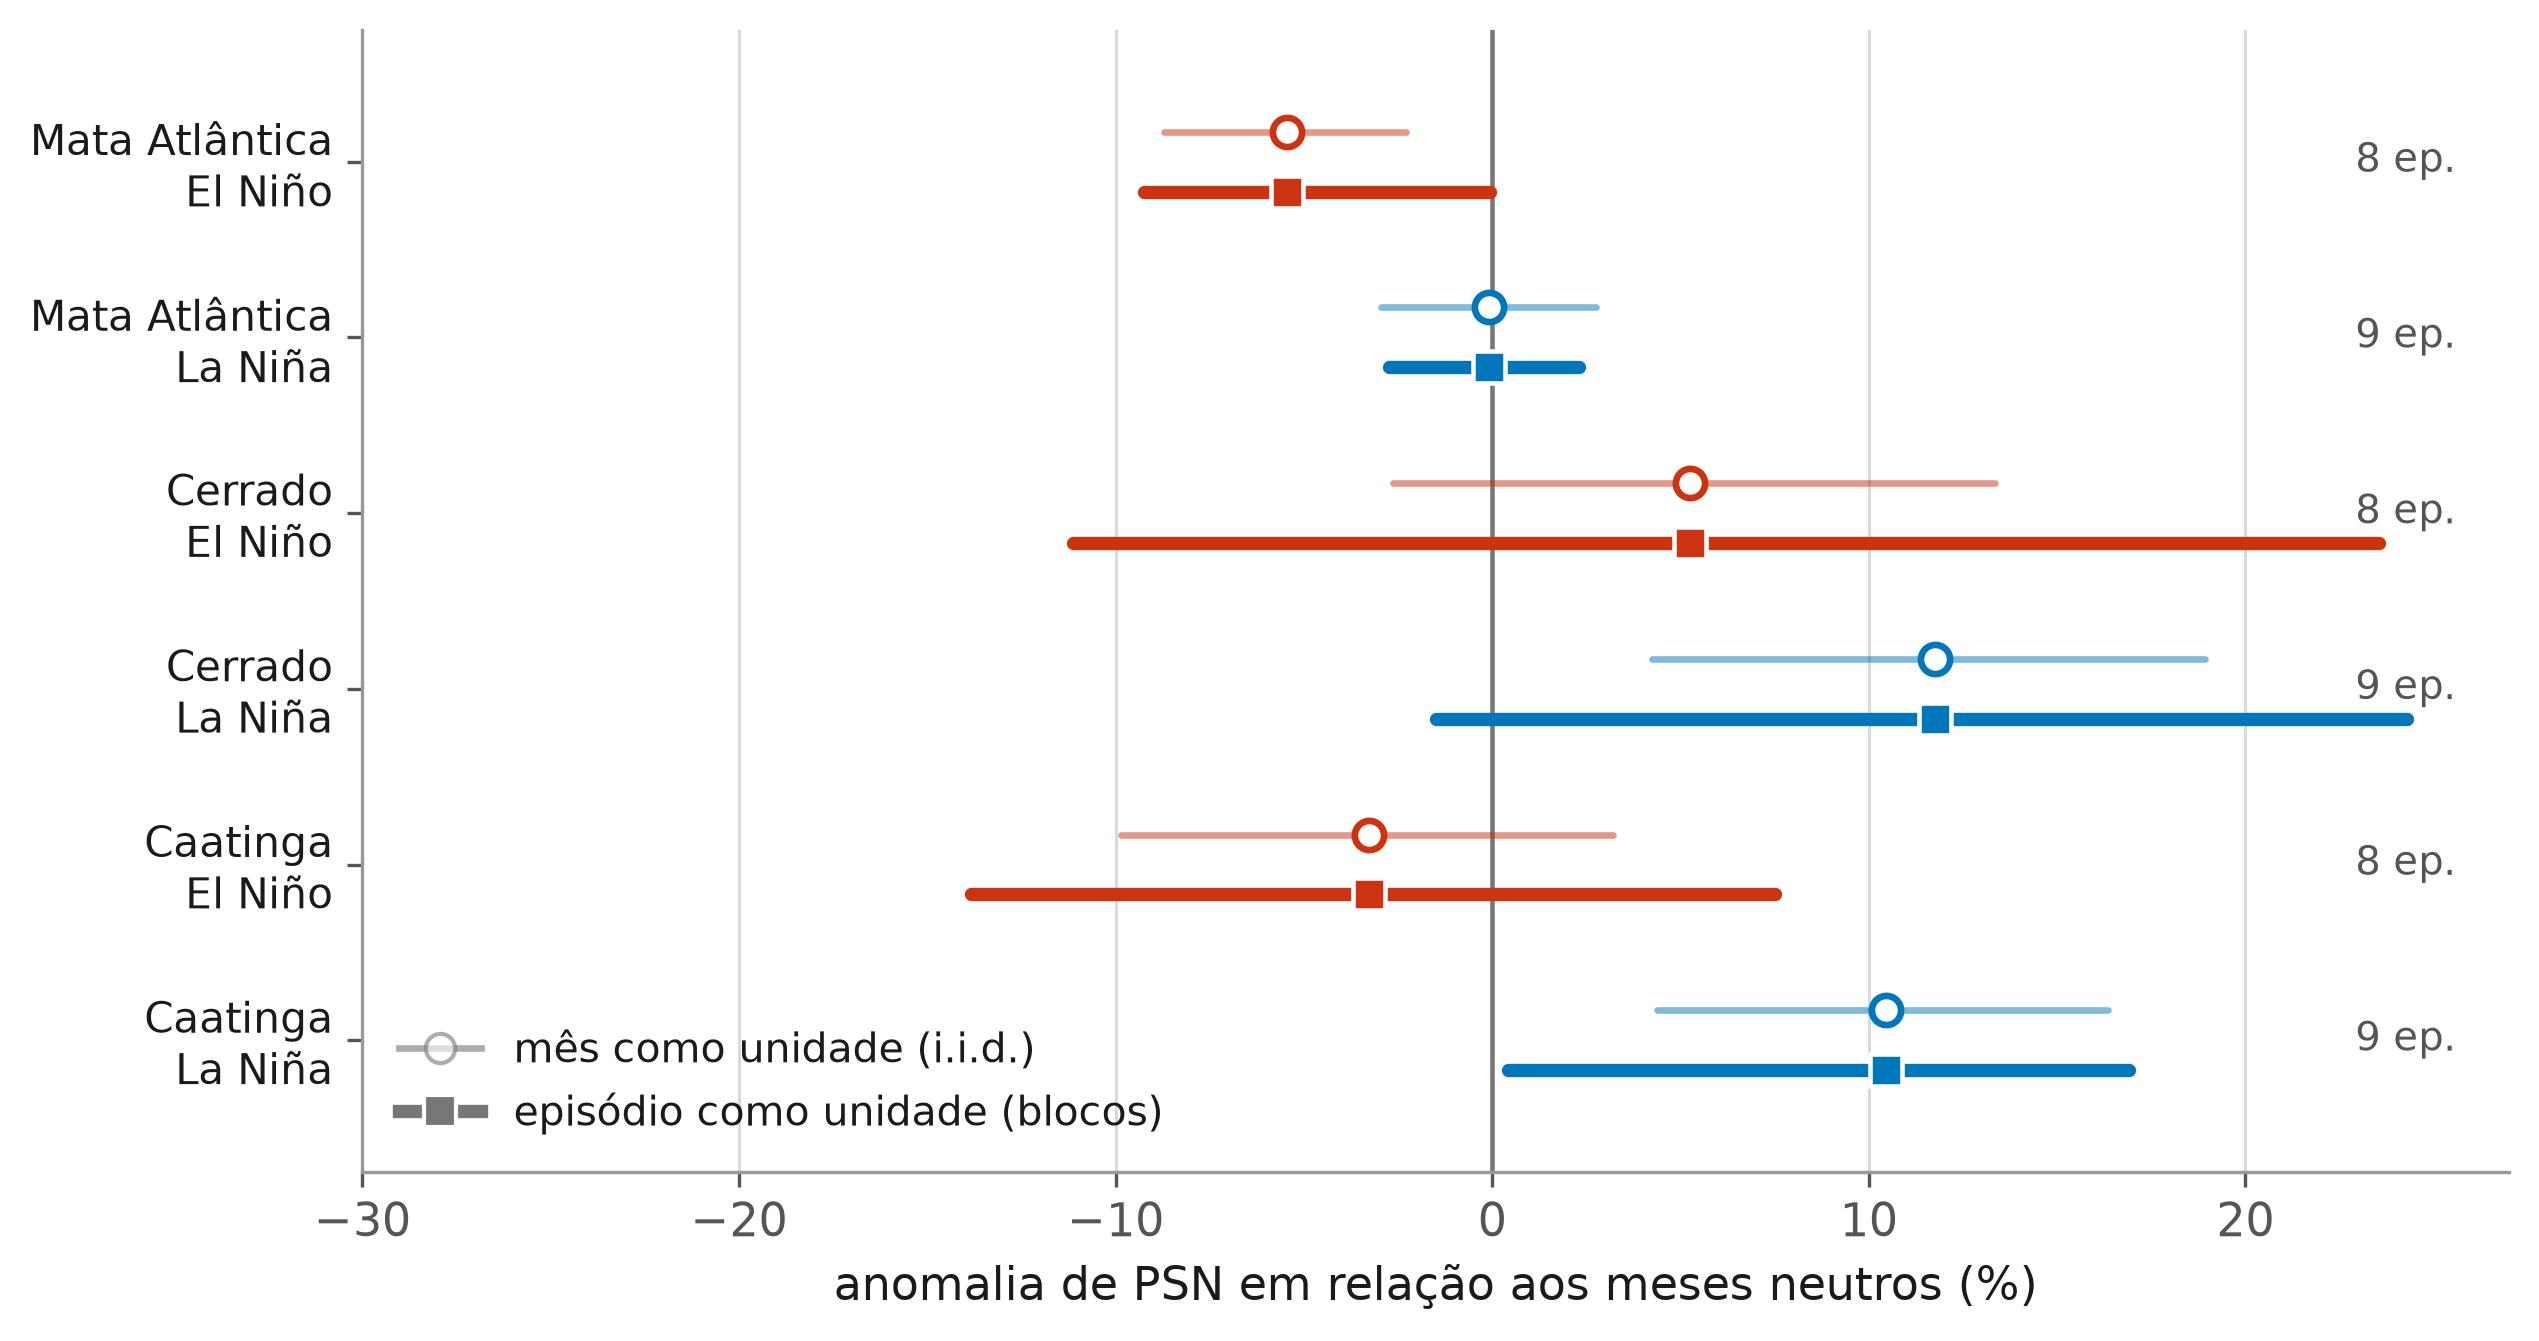
\includegraphics[width=\linewidth]{figs/fig2_unidade.png}
\caption{Anomalia de PSN de cada fase em relação aos meses neutros, com intervalos de confiança de 95\% obtidos por bootstrap sobre meses (linha fina, círculo aberto) e por bootstrap em blocos sobre episódios (linha grossa, quadrado). O número de episódios de cada fase consta à direita.}
\label{fig:unidade}
\end{figure}

Nenhum resultado troca de sinal entre os dois esquemas, e o contraste entre os biomas descrito nas Seções~3.2 a 3.4 mantém-se. O que a verificação estabelece é que a magnitude de cada anomalia é estimada com precisão limitada pelo número de episódios disponíveis, e não pelo número de meses, e que essa precisão não basta para sustentar qualquer efeito isolado sob controle de comparações múltiplas na análise agregada. A exceção é a análise sazonal da Seção~3.6, em que a concentração do sinal na estação chuvosa eleva a magnitude o suficiente para que a resposta da Caatinga sobreviva à correção em ambas as famílias de testes.

\section{Discussão}

\subsection{Padrões contrastantes ao longo do gradiente hidroclimático}

Os três biomas respondem ao mesmo forçante remoto de maneiras distintas, e a diferença acompanha o fator que limita a produtividade de cada um. Na Mata Atlântica, bioma úmido em que a água raramente é limitante, o sinal do ENSO chega sobretudo como anomalia térmica e a associação com a produtividade aparece na fase quente. No Cerrado e na Caatinga, limitados pela água, o sinal aparece no balanço hídrico e a associação surge na fase fria. Os dois biomas sazonais compartilham o canal, mas não o tempo de resposta: a Caatinga responde em fase e por pouco tempo, o Cerrado de forma fraca e persistente.

O confinamento sazonal reforça essa leitura. A associação com a La Niña é detectada no trimestre chuvoso e não no seco, e sua magnitude no trimestre chuvoso cresce ao longo do gradiente, de 7,4~p.p.\ na Mata Atlântica a 25,0~p.p.\ na Caatinga. É o padrão que se esperaria de um canal hídrico: o excedente de água só pode se converter em produtividade onde e quando há água a ser modulada, e seu efeito relativo é tanto maior quanto mais o sistema seja limitado por ela. Convém, porém, não confundir a ausência de detecção no trimestre seco com a demonstração de que as duas estações diferem: o contraste direto entre elas só é conclusivo na Mata Atlântica, e na Caatinga, apesar da maior magnitude, a diferença entre os trimestres não se distingue de zero.

As escalas de resposta temporal completam o quadro e, ao contrário das correlações com o ONI, separam os biomas com nitidez. A Caatinga é o único cuja produtividade se associa à chuva do próprio período, tem a associação mais forte de todas na janela de quatro períodos e a perde mais depressa; o Cerrado tem a curva mais achatada, retendo 88\% do máximo doze períodos depois. A Figura~\ref{fig:conceitual} resume os três padrões.

\begin{figure}[pos=!ht]
\centering
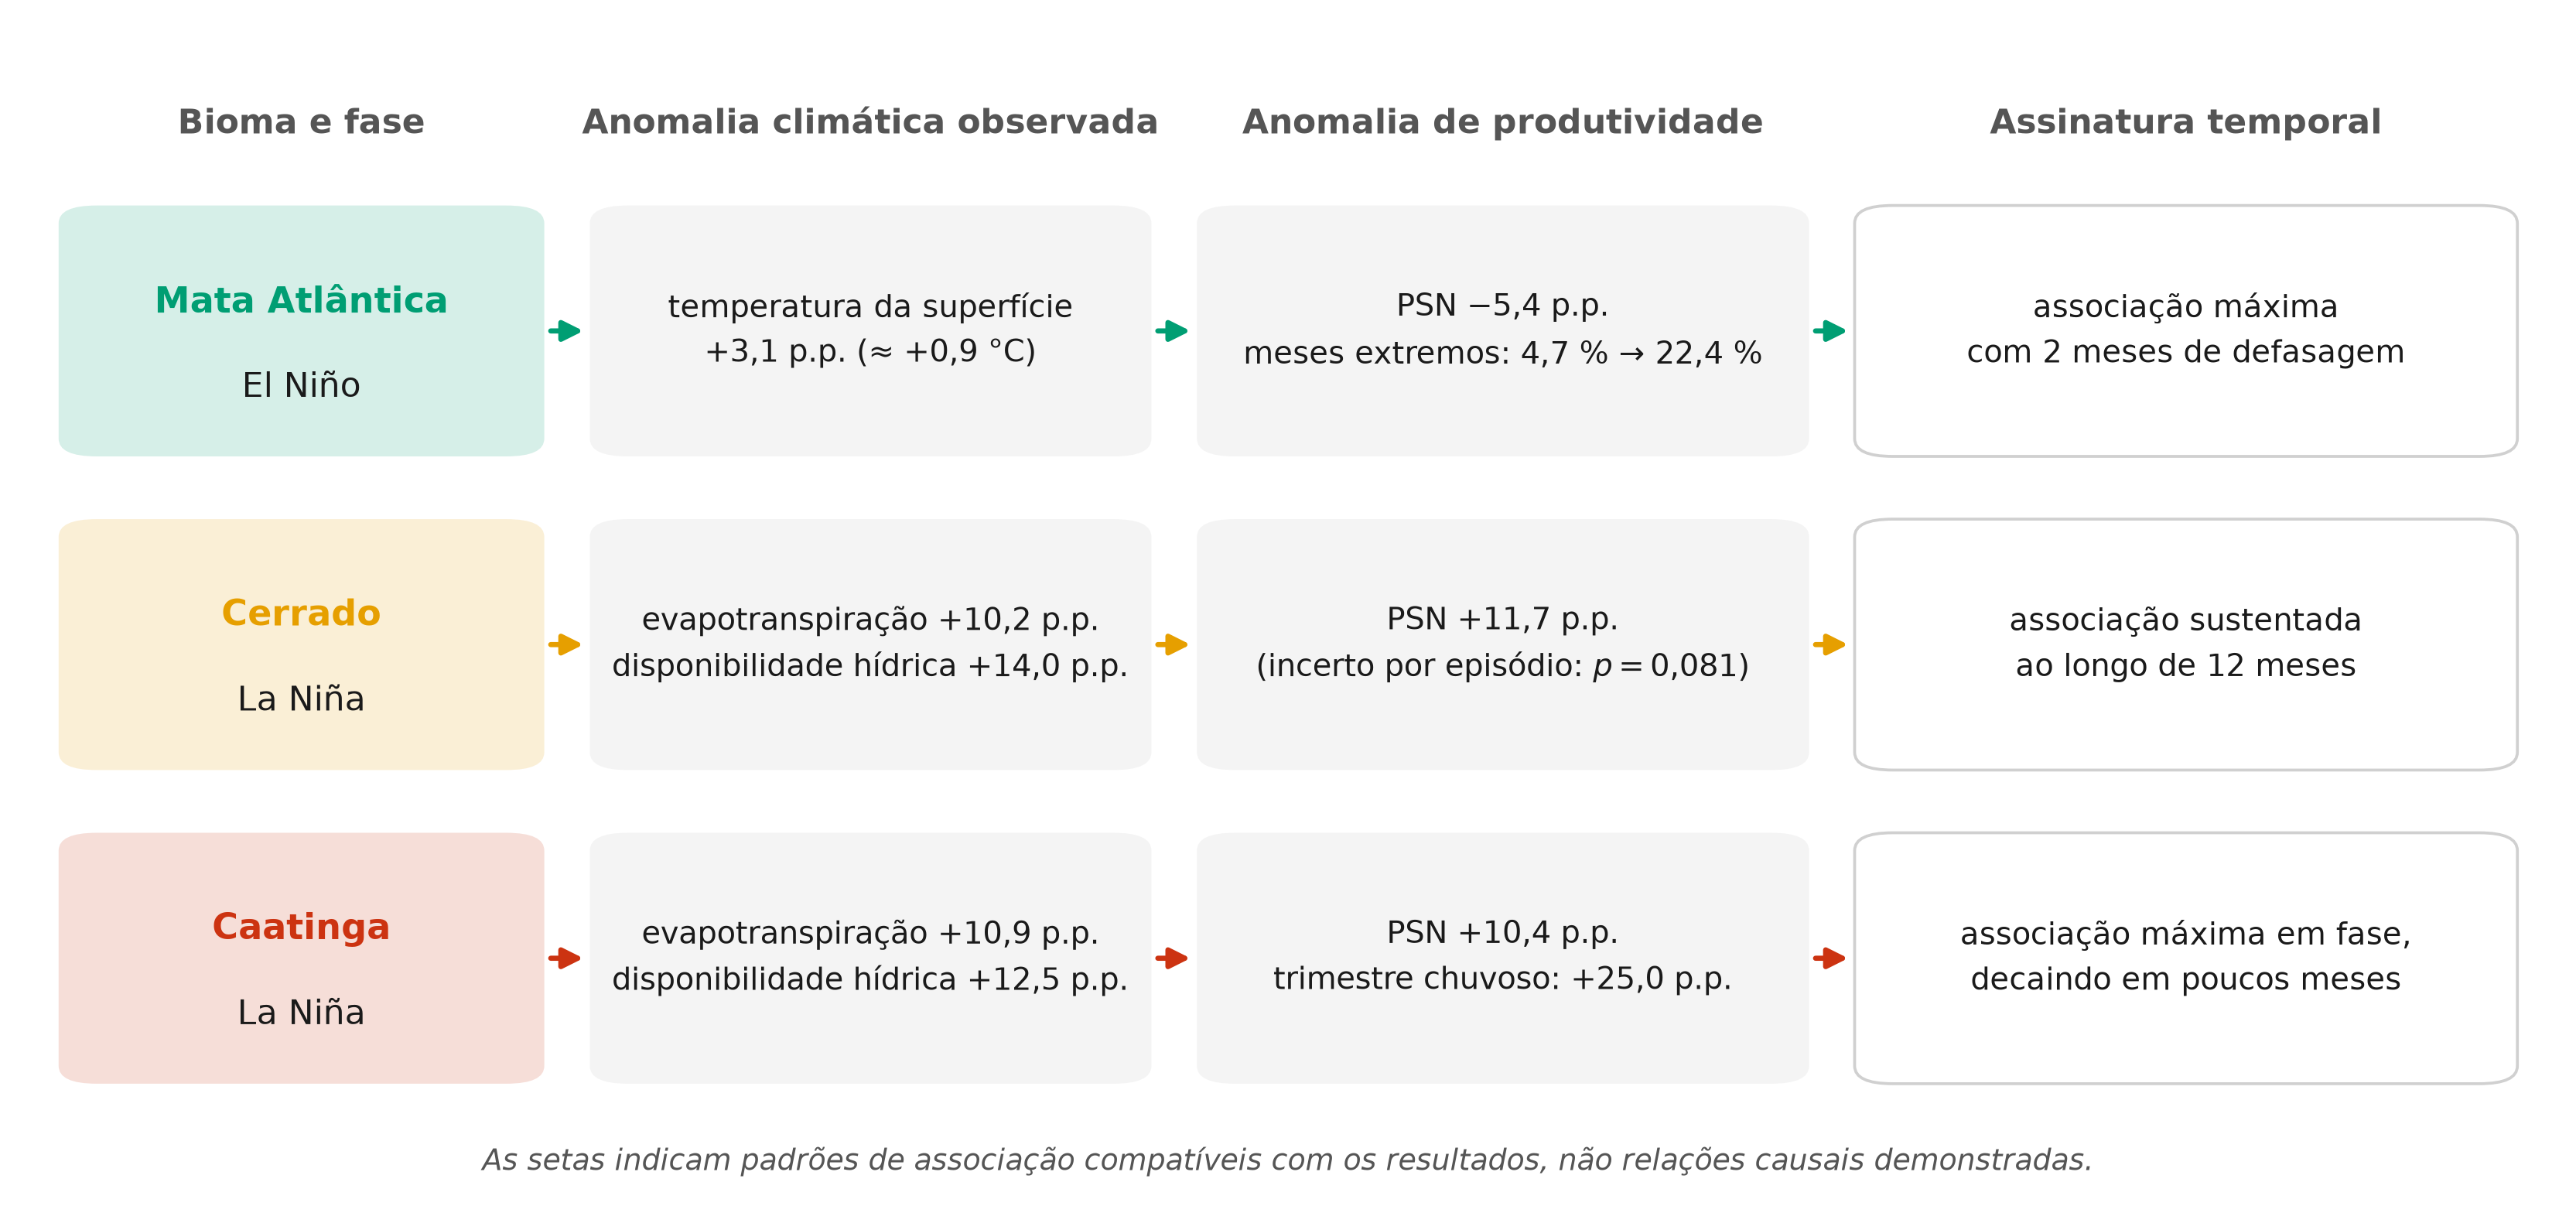
\includegraphics[width=\linewidth]{figs/fig5_conceitual.png}
\caption{Síntese dos três padrões de associação observados. As setas indicam encadeamentos compatíveis com os resultados, não relações causais demonstradas.}
\label{fig:conceitual}
\end{figure}

\subsection{O sinal térmico na Mata Atlântica}

Na Mata Atlântica, o El Niño associa-se a uma superfície cerca de 0,9~$^{\circ}$C mais quente que o normal da época, e essa é a anomalia climática mais robusta de todo o estudo: é o único efeito que mantém $p$ abaixo de 0,05 quando o episódio passa a ser a unidade amostral. A teleconexão do ENSO com o Leste do Nordeste brasileiro é, de fato, mais consistente na temperatura do que na precipitação \citep{ropelewski1987, kayano2007}, e a sensibilidade da fotossíntese à demanda evaporativa em florestas tropicais úmidas é bem documentada \citep{lawson2019, vourlitis2022}. O padrão observado é consistente com estresse térmico e evaporativo durante a fase quente.

Dois aspectos merecem cautela. O primeiro é que o canal térmico é o maior canal isolado do experimento de perturbação nesse bioma, mas por pouca margem sobre a evapotranspiração, e a temperatura é o preditor de menor importância por permutação no modelo ajustado para a Mata Atlântica \citep{oliveira2026}. A leitura defensável não é a de que o modelo seja térmico, e sim a de que a anomalia climática associada ao ENSO nesse bioma se concentra na temperatura, de modo que é por esse canal que a maior parte da resposta reproduzida se dá. O segundo é que a associação concentra-se na cauda inferior da distribuição: as medianas brutas são indistinguíveis entre fases e o que muda é a frequência de meses extremamente baixos, que quase quintuplica. Um teste de posição central aplicado a valores brutos não detectaria esse padrão, e descrevê-lo como uma redução média da produtividade seria enganoso.

\subsection{Integração hídrica e resposta persistente no Cerrado}

No Cerrado, o sinal associado à La Niña aparece na evapotranspiração e na disponibilidade hídrica, e não na precipitação do próprio período. Essa dissociação é coerente com a fisiologia envolvida: transpiração e assimilação ocorrem pelos mesmos estômatos \citep{lawson2019}, de modo que a água efetivamente utilizada informa sobre a produtividade melhor do que o total que caiu no período. A precipitação é um fluxo de entrada ruidoso, e a vegetação responde à água que permaneceu disponível no solo nas semanas seguintes \citep{oliveira2005, schwinning2004}.

A estrutura temporal aponta na mesma direção, e a associação com a água acumulada é mais informativa a esse respeito do que a correlação com o ONI. Esta última mantém-se de intensidade semelhante ao longo de doze meses, sem pico bem definido, mas é fraca demais (não ultrapassa 3,6\% da variância) para que dela se derive um tempo de resposta. Já a associação com a chuva acumulada é forte e tem forma característica: praticamente nula na janela de um período ($\rho = 0{,}09$), cresce até um máximo em cinco períodos e mantém 88\% desse máximo doze períodos depois, a curva mais achatada dos três biomas. O Cerrado é, assim, o bioma em que a produtividade menos responde à chuva recente e mais responde à água acumulada ao longo de quase um ano.

Essa assinatura é compatível com a capacidade de integração hídrica atribuída às savanas do Brasil Central, em que sistemas radiculares profundos acessam água armazenada em profundidade e amortecem a variabilidade de curto prazo da chuva \citep{oliveira2005, bucci2008}. A chuva acumulada é, contudo, um substituto da água efetivamente armazenada no solo, e não a sua medida; a interpretação é ecologicamente compatível com o padrão observado, não um mecanismo demonstrado.

Duas limitações específicas devem acompanhar a leitura do Cerrado. A primeira é que a evapotranspiração e a disponibilidade hídrica compartilham grande parte da informação nesse bioma \citep{oliveira2026}, de modo que seus canais não são separáveis no experimento de perturbação; a soma dos canais isolados não corresponde à resposta do conjunto. A segunda é que o aumento de PSN em La Niña, embora seja o maior da análise agregada, deixa de ser distinguível de zero quando as nove sequências de La Niña são tratadas como unidades independentes ($p = 0{,}081$). O Cerrado apresenta, portanto, um padrão positivo consistente na direção, mas com elevada incerteza sob inferência por episódio.

\subsection{Resposta em pulso na Caatinga}

Na Caatinga, a associação com a La Niña é a mais imediata e a mais forte do conjunto. A correlação com o ONI é máxima em fase e decai em poucos meses; mais nítido ainda, é o único bioma cuja produtividade se associa à chuva do próprio período ($\rho = 0{,}32$, contra 0,09 no Cerrado e praticamente zero na Mata Atlântica), atinge a associação mais alta de toda a análise na janela de quatro períodos ($\rho = 0{,}67$) e retém apenas 69\% dela doze períodos depois. A anomalia de PSN restrita ao trimestre chuvoso alcança 25,0~p.p., o único resultado do estudo que sobrevive à correção para comparações múltiplas em qualquer família de testes considerada. O padrão é compatível com a dinâmica de pulsos de recursos característica de ecossistemas semiáridos, em que a atividade biológica responde rapidamente aos eventos de disponibilidade de água e retorna com igual rapidez ao estado basal \citep{schwinning2004}, e com o que registram as medições de fluxo de carbono na Caatinga, que acompanham a magnitude e a distribuição da chuva \citep{mendes2020, mendes2025}. O experimento de perturbação é coerente com esse quadro: a evapotranspiração sozinha reproduz a maior parte da anomalia observada, e o conjunto dos preditores reproduz 9,8 dos 10,4 pontos percentuais observados.

Que a resposta seja maior no bioma mais seco é o que se esperaria de um sistema em que a água é o fator limitante dominante: a mesma anomalia hídrica relativa produz maior variação relativa de produtividade onde a produtividade basal é mais baixa e mais dependente de água.

\subsection{Implicações para o monitoramento da produtividade}

O contraste entre os três biomas tem consequências práticas para o acompanhamento de anomalias de produtividade por sensoriamento remoto na região, e a principal delas é que não há um indicador único adequado aos três.

Nos biomas limitados pela água, a variável de acompanhamento mais informativa é a água acumulada, e não a chuva do período nem o índice oceânico. A chuva do próprio período não distingue as fases do ENSO em nenhum dos três biomas depois de removido o ciclo anual, e o ONI explica menos de 4\% da variância das anomalias; a chuva acumulada, ao contrário, alcança correlações entre 0,48 e 0,67. A janela de acumulação, porém, deve ser escolhida por bioma: quatro a cinco períodos captam o máximo em todos, mas uma janela curta é suficiente na Caatinga e insuficiente no Cerrado, onde a associação persiste por quase um ano.

No bioma úmido, a variável de acompanhamento mais informativa é térmica, e o alvo do monitoramento não é a média. Na Mata Atlântica o El Niño desloca pouco o centro da distribuição de produtividade e muda muito a sua cauda inferior, o que significa que um sistema de alerta baseado em médias mensais tenderia a não detectar o efeito que mais importa. Indicadores de frequência de meses extremamente baixos são, nesse caso, mais adequados do que indicadores de anomalia média.

Por fim, a escala anual não substitui a mensal. Nenhum bioma apresentou tendência interanual significativa, e os anos extremos não coincidem com as fases do ENSO de forma sistemática, porque um ano civil mistura meses de fases distintas e, no caso dos biomas sazonais, dilui em doze períodos um sinal que se concentra em três.

\subsection{Dependência temporal e limites da inferência}

Em 24 anos há 8 episódios de El Niño e 9 sequências de La Niña, com duração mediana de 8 meses. Blocos dessa duração fazem o tamanho amostral efetivo ser uma fração do nominal, e o erro-padrão cresce aproximadamente com a raiz dessa razão; o alargamento mediano de 1,67 vez nos intervalos é o que se esperaria dessa aritmética, e não um efeito peculiar a esta série. A consequência é que a análise agregada, embora descreva padrões coerentes e de sinal estável, não sustenta nenhum efeito isolado após correção para comparações múltiplas. A leitura adequada não é a de que não exista associação, nem a de que o ENSO tenha sido estabelecido como causa: é a de que há um padrão climaticamente coerente estimado com baixa precisão inferencial, por escassez de episódios independentes.

A estratificação sazonal é a exceção parcial, e pela razão certa: ao restringir a análise à estação em que o canal hídrico pode operar, a magnitude do efeito cresce o suficiente para superar o alargamento dos intervalos. Ela deve, ainda assim, ser lida como estratificação motivada pelo mecanismo e não como teste pré-registrado, e sua robustez depende da família de testes adotada, como reportado na Seção~3.5.

Outras limitações devem ser explicitadas. A classificação em três fases descarta a intensidade dos episódios, que varia de um ONI de pico de 0,71 a 2,59 na série. A análise é correlacional e não separa o ENSO de outros modos de variabilidade que possam coincidir com ele no período, como a Oscilação Decadal do Pacífico \citep{kayano2007}. A PSN e a evapotranspiração provêm de algoritmos MODIS que compartilham entradas, de modo que o experimento de perturbação não constitui evidência independente; na Mata Atlântica em La Niña, aliás, ele prediz sinal oposto ao observado, ainda que ambos sejam próximos de zero. A unidade temporal é uma janela de cerca de 32 dias atribuída a um mês de referência, e não o mês civil. Por fim, a temperatura da superfície não passou por filtro de qualidade pela banda QC\_Day, e a sensibilidade da série a esse filtro não foi avaliada.

Duas direções decorrem do exposto. A primeira é elevar o número de unidades independentes, estendendo a série para trás do início do registro MODIS ou analisando sub-regiões dentro de cada bioma em vez de uma única média por bioma. A segunda é metodológica: compósitos de fase do ENSO construídos sobre séries mensais ganham em transparência quando acompanhados de inferência que respeite a estrutura temporal, seja por bootstrap em blocos, por testes de permutação sobre rótulos de episódio ou por correção do tamanho amostral efetivo \citep{kunsch1989, politis1994}, cujo custo computacional é baixo.

\section{Conclusões}

As fases do ENSO associam-se a padrões distintos de fotossíntese líquida ao longo do gradiente hidroclimático da Bahia, e o contraste entre os três biomas acompanha o fator que limita a produtividade de cada um.

Na Mata Atlântica, os resultados são consistentes com uma via térmica: o El Niño associa-se a uma superfície cerca de 0,9~$^{\circ}$C mais quente e a uma quase quintuplicação da frequência de meses de produtividade extremamente baixa, sem deslocamento das medianas. No Cerrado e na Caatinga, os padrões relacionam-se ao balanço hídrico durante a La Niña, com anomalias positivas de evapotranspiração e de disponibilidade hídrica acompanhando aumentos de PSN de 11,7 e 10,4 pontos percentuais, e sem sinal na precipitação do próprio período. Os dois diferem no tempo, e a diferença aparece com clareza na janela de acumulação da chuva: a Caatinga é o único bioma cuja produtividade se associa à chuva do próprio período e o que mais rapidamente perde essa associação, enquanto o Cerrado retém 88\% do seu máximo doze períodos depois.

A associação com a La Niña é detectada na estação chuvosa e não na seca, e sua magnitude cresce na direção do polo semiárido, de 7,4 a 25,0 pontos percentuais; o contraste direto entre as estações, porém, só é conclusivo na Mata Atlântica.

Esses padrões têm consequência prática: não há um indicador único de monitoramento adequado aos três biomas. Nos biomas limitados pela água a variável mais informativa é a chuva acumulada, com janela escolhida por bioma; no bioma úmido é a temperatura, e o alvo não é a anomalia média, e sim a frequência de meses extremamente baixos. O experimento de perturbação com o modelo reproduz de 57\% a 94\% da magnitude observada nas combinações de maior efeito, o que indica compatibilidade entre as anomalias climáticas observadas e as anomalias de produtividade, sem estabelecer transmissão causal.

Há, contudo, poucos episódios independentes em 24 anos. Sob inferência por episódio, os intervalos alargam-se 1,67 vez em mediana e nenhum efeito isolado da análise agregada permanece após correção para comparações múltiplas; apenas a resposta da Caatinga na estação chuvosa sobrevive. O estudo identifica, portanto, padrões climáticos e ecológicos coerentes ao longo do gradiente, cuja confirmação individual exigirá séries mais longas ou maior replicação espacial.

\section*{Disponibilidade de dados}
A base mensal (297 períodos por bioma, 2001--2025), o código em Python das análises aqui reportadas e os resultados da rodada completa estão disponíveis em \url{https://github.com/heroslore/MRMP-N-PSN-Bahia} e arquivados de forma permanente no Zenodo sob o DOI \url{https://doi.org/10.5281/zenodo.22883915}, que resolve sempre para a versão mais recente do arquivo. A base é também fornecida como material suplementar (arquivo CSV).

\section*{Declaração de conflito de interesses}
Os autores declaram não haver conflitos de interesse financeiros ou pessoais que pudessem ter influenciado o trabalho relatado neste artigo.

\section*{Agradecimentos}
O presente trabalho foi realizado com apoio da Coordenação de Aperfeiçoamento de Pessoal de Nível Superior -- Brasil (CAPES) -- Código de Financiamento 001, por meio de bolsa de mestrado concedida ao primeiro autor. Os autores agradecem ao Programa de Pós-graduação em Ciências e Tecnologias Ambientais (UFSB/IFBA). O primeiro autor agradece ao Prof. Dr. Fabrício Berton Zanchi, pela orientação, e à Profa. Dra. Nayanne Silva Benfica, pela coorientação.

\section*{CRediT authorship contribution statement}
\textbf{Ygor Augusto dos Santos Oliveira:} Conceituação, Metodologia, Software, Análise formal, Curadoria de dados, Redação -- rascunho original. \textbf{Nayanne Silva Benfica:} Conceituação, Metodologia, Curadoria de dados, Redação -- revisão e edição, Supervisão. \textbf{Fabrício Berton Zanchi:} Conceituação, Metodologia, Redação -- revisão e edição, Supervisão.

\bibliographystyle{cas-model2-names}
\bibliography{refs2}

\end{document}
